% !TeX spellcheck = en_US
% Recommended reading:
\begin{frame}
	Recommended reading for this section:
	\begin{itemize}
		\item Lectures 1,2,3 in \cite{TreBau}
		\item Sections I.1, I.2, I.3, I.5(, I.11) in \cite{StrangData}
		\item Chapters 1,3(,4,5) in \cite{StrangLA_intro}
	\end{itemize}
	
	\bibliographystyle{plain}
	~\\~\\
	Literature:\\
	\bibliography{../information/literature.bib}
\end{frame}


\begin{frame}
\Vspace{0.2cm}
\Section{Fundamentals of Linear Algebra}
\Subsection{Matrices and Vectors}
\begin{example}[Interpolation] \label{ex:interpolation}
	 ~\\
	Assume we are given the following measurements
	\begin{table}
		\begin{tabular}{c|ccc}
			$z_i$ &-1&0&1\\
			\hline
			$y_i$  &0&1&0
		\end{tabular}
	\end{table}
	We postulate that these measurements can be explained exactly by the (quadratic) model
	$$f(z):=f_{x}(z) := x_1 + x_2 z^2 .$$
	Question: Can we find parameters $x_1,x_2 \in \R$, so that $f(z_i) = y_i$ for all $i=1,\ldots,3$?\\~\\
	\Hide{
		We first translate the task into the following system of \textit{linear} equations:
		\begin{equation*}
		\begin{array}{crcl}
	i=1:	&1x_1 + 1x_2 &=&0\\
	i=2:	&1x_1 +0x_2 &=&1\\
	i=3:	&1x_1 +1x_2 &=&0
		\end{array}
		\ \Leftrightarrow: \
		\underbrace{
			\begin{pmatrix}
			1 & 1 \\ 
			1& 0  \\ 
			1 & 1 
			\end{pmatrix}
		}_{A}
		\cdot
		\underbrace{
			\begin{pmatrix}
			x_1 \\ x_2  
			\end{pmatrix}
		}_{x}
		=
		\underbrace{
			\begin{pmatrix}
			0\\ 1 \\ 0
			\end{pmatrix}
		}_{b}
		\ \Leftrightarrow \
		Ax=b
		\end{equation*}
		Why linear? Roughly speaking, because the $x_i$ only appear with power $1$ and there are no combinations $x_ix_j$.\\~\\
		Also note, the abstracting notation $Ax=b$ provides a rigorous interface to analyze this problem theoretically and also to implement numerical solvers. ~\\~\\
		\demo{solve and draw points}
	} 
\end{example}
\end{frame}


\begin{frame} 
Throughout we will consider matrices over  $\F \in \{\R,\C\}$. However, $\F$ could be replaced by any \href{https://en.wikipedia.org/wiki/Field_(mathematics)}{field}.\\
\begin{defi}[Matrix] \label{def:matrix} 
	\unitlength1cm 
	\begin{picture}(15,0) 
%	\put(10,-3){\includegraphics{LocalFolder/LocalMedia/3_a-indices}} 
	\end{picture} 
	Let $m,n \in \mathbb{N}$. Then a rectangular array of numbers in $\F $ with $m$ \textit{rows} and $n$ \textit{columns}, written as
%	$A: \{1,\ldots, m\} \times \{1, \ldots, n\} \to \F$ represented by the array 
	\begin{eqnarray*} 
		A= (a_{ij})_{ij} = \left(  \begin{array}{cccc} 
			a_{11} & a_{12} & \cdots & a_{1n} \\ 
			a_{21} & a_{22} & \cdots & a_{2n} \\ 
			\vdots & \vdots &        & \vdots \\ 
			a_{m1} & a_{m2} & \cdots & a_{mn} \end{array} \right),
	\end{eqnarray*} 
%	with $a_{ij} \in \F$ for all $i=1,...,m$, $j=1,...,n$
	 is called a  
	{\bf $(m\times n)$ matrix} {\bf with coefficients in $\F$}. \\[4pt]
	\vspace{0.2cm} 
	\Hide{\small
		\begin{tabular}{@{}ll} 
			$\F^{m\times n}$: & set of all $(m\times n)$ matrices with coefficients in  $\F$ \\[0.1cm] 
			$\F^{n} := \F^{n\times 1}$: &matrices with just one column are called (column) \textbf{``vectors''};\\ 
			&elements in $\F^{1\times n}$ are referred to as row vectors \\[0.1cm] 
			$a_{ij}$:        & the $(i,j)$-th {\bf coefficient} or {\bf 
				entry} \\[0.1cm] 
			$(a_{i1},...,a_{in})$: & the $i$-th {\bf row} of $A$ (this is a  
			$(1\times n)$-matrix, , $n$-dimensional vector) \\[0.4cm] 
			$\begin{pmatrix}  a_{1j} \\ \vdots \\ a_{mj}  
			\end{pmatrix}:$ 
			& the $j$-th {\bf column} of $A$ (this is a $(m\times 1)$-matrix, $m$-dimensional vector)
			\\[0.8cm] 
			$0$: & the {\bf zero matrix} or {\bf null matrix}, i.e. all entries $0$ \\[0.1cm] 
			$I_n$: & the  \textbf{unity} or \textbf{identity matrix} in $\F^{n\times n}$, i.e. the Matrix with 
			entries \\ 
			& $\delta_{ij} = \begin{cases} 1, \quad\text{ if }i=j \\ 0, \quad \text{ else} 
			\end{cases}$ ({\footnotesize ``Kronecker delta''}), \quad\text{i.e.}\quad $I_n = \begin{pmatrix} 
			1 & 0 & \cdots & 0\\ 
			0 & & \ddots & \vdots \\ 
			\vdots & \ddots & \ddots & 0 \\ 
			0 & \cdots & 0 & 1  
			\end{pmatrix}$ 
		\end{tabular} 
	}
\end{defi} 
\end{frame}


%OPERATIONS with matrices
\begin{frame}
 \textbf{Operations}~\\
% 
We can add  matrices of same size and scale the entries of a matrix.\\
\Hide{~\\
\begin{ex}[Summing and scaling matrices]
	\begin{align*}
	\begin{pmatrix}2&1\\0&-1\end{pmatrix}
	&+\begin{pmatrix}1&-1\\1&0\end{pmatrix} 
	:=\begin{pmatrix}3&0\\1&-1\end{pmatrix}\\
	2\cdot\begin{pmatrix}2&1\\0&-1\end{pmatrix} 
	&=\begin{pmatrix}2\cdot2&2\cdot1\\2\cdot0&2\cdot(-1)\end{pmatrix}
	:=\begin{pmatrix}4&2\\0&-2\end{pmatrix}
	\end{align*}
\end{ex}
}
%	
\begin{defi}[Summing and scaling matrices]\label{def:sum_scale_mats}
	Let $A,B\in\F^{m\times n}$ be matrices, $m,n \in \N$ and $r \in \F$.
	\vspace{0.2cm}
	\begin{itemize}
		\item[i)] \textbf{Sum of matrices:} $+\colon \F^{m\times n} \times \F^{m\times n} \to \F^{m\times n}$\\ \vspace{0.1cm}
		The sum $C := A + B$ of the two matrices $A$ and $B$ is defined to be the matrix $C= (c_{ij})_{ij} \in \F^{m\times n}$ with entries
		\[
		c_{ij} := a_{ij} + b_{ij}\text{~~~for~~~}i=1,...,m,~ j=1,...,n .
		\]
		\vspace{0.2cm}
		\item[ii)] \textbf{Multiplication with scalars:} $\cdot\colon \F  \times \F^{m\times n} \to \F^{m\times n}$\\ \vspace{0.1cm}
		The product of the matrix $A$ with $r\in\F $ is defined to be the scaled matrix $$r\cdot A := (r\cdot a_{ij})_{ij}.$$
		In this context, elements of the field $\F $ are called \textbf{scalars}.
	\end{itemize}
\end{defi}
\end{frame}



%EXAMPLE: sum and product of matrices
\mode<article>{
\begin{frame} 
\begin{re}~\\
-- why did we need a field $\F $?\\
-- think of $+\colon \F^{m\times n} \times \F^{m\times n} \to \F^{m\times n}$ being an operation on $\F^{m\times n}$\\
Then Because of the entrywise definition, the matrix sum inherits group properties $(G,+)$ from the field $\F $. \\
-- scalar = element of $\F $, think of $\R$
\end{re}

\begin{ex}
\end{ex}
\end{frame}
}



\begin{frame}
	\Hide{\small
\textbf{Question:} How do summing and scaling get along in a mixed expression?\\
We can prove the following rules:\\
\begin{lemma}[Compatibility properties of summing and scaling] \label{lem:compatibility_sum_scale}
	Let $A,B \in \F^{m\times n}$ and $r,s \in \F $. Then 
	\begin{eqnarray*} 
		\begin{array}{lr@{~}l} 
			i) & (r\cdot s) \cdot A = & r\cdot(s\cdot A)  \hspace*{10cm} \\ 
			ii) & (r+s) \cdot A =      & r\cdot A+s\cdot A  \\ 
			~ & r\cdot (A+B) =       & r \cdot A+r \cdot B  \\ 
			iii) & 1\cdot A = & A  
		\end{array}  
	\end{eqnarray*}
\end{lemma}
%
\begin{proof}\blank
	Follow immediately from Definition \ref{def:sum_scale_mats} in terms of matrix coefficients and the field properties of $\F $. For example:
	\begin{itemize}
		\item[i)] $(r\cdot s)A = [(r\cdot s) a_{ij}]_{ij} \stackrel{{(\tiny \text{associativity in} \F)}}{=} [ r\cdot (s \cdot a_{ij})]_{ij} = r \cdot (s\cdot A)$
		\item[ii)]$(r + s)A = [(r + s) a_{ij}]_{ij} \stackrel{{(\tiny \text{distributivity in} \F)}}{=} [ ra_{ij} + sa_{ij}  ]_{ij} = r\cdot A+s\cdot A$
	\end{itemize} 
\end{proof} 
\begin{re}
	One can show that $(\F^{m\times n}, +)$ is a so--called abelian group. Then the compatibility properties from Lemma \ref{lem:compatibility_sum_scale} imply that $(\Fmn, +,\cdot)$ is a so-called {\color{defgruen} \text{vector space} (over $\F $)}.
\end{re}
~\\
From Lemma \ref{lem:compatibility_sum_scale} we can deduce further properties of $(\Fmn, +,\cdot)$.
\begin{corollary}
	Let $A  \in \F^{m\times n}$ and $r  \in \F $. Then
	\begin{eqnarray*} 
		\begin{array}{lr@{~}l} 
			i)& 0 \cdot A &= 0 \\
			ii)& r \cdot 0 & = 0 \\
			iii)& r\cdot A &= 0 ~~ \Rightarrow r = 0 ~\lor ~A = 0\\ 
			iv) & (-1)\cdot A &=    -A ~~~~~~\text{(i.e., $(-1)\cdot A$ is the additive inverse of $A$)}
		\end{array}  
	\end{eqnarray*}
\end{corollary}
\begin{proof} 
	\blank
	Follows from Lemma \ref{lem:compatibility_sum_scale} and the field properties of $\F $. For example:\\[0.2cm]
	iv) To show: $(-1)\cdot A  + A = 0$. We find 
	$$(-1)\cdot A  + A \stackrel{\text{(L.\ref{lem:compatibility_sum_scale} iii))}}{=} (-1)\cdot A  + 1\cdot  A \stackrel{\text{(L.\ref{lem:compatibility_sum_scale} (ii))}}{=} (-1 + 1)\cdot A = 0\cdot A \stackrel{\text{(i)}}{=} 0. $$
\end{proof}
}
 \end{frame}


\begin{frame} 
Next we provide a notation which enables us to write linear systems of equations in a concise way.\\
We recall from Example \ref{ex:interpolation}:
\begin{equation*}
\begin{array}{rcl}
1x_1 + 1x_2 &=&0\\
1x_1 +0x_2 &=&1\\
1x_1 +1x_2 &=&0
\end{array}
\ \Leftrightarrow: \
\underbrace{
	\begin{pmatrix}
	1 & 1 \\ 
	1& 0  \\ 
	1 & 1 
	\end{pmatrix}
}_{A}
\cdot
\underbrace{
	\begin{pmatrix}
	x_1 \\ x_2  
	\end{pmatrix}
}_{x}
=
\underbrace{
	\begin{pmatrix}
	0\\ 1 \\ 0
	\end{pmatrix}
}_{b}
\ \Leftrightarrow \
Ax=b
\end{equation*}
\begin{defi}[Matrix-Vector Product]
 Let $A \in \F^{m\times n}$ and $x\in \F^n$. Then the \textbf{\color{defgruen} matrix-vector product $b=Ax \in \F^m$} is defined by
\[
b_i=a_{i1}x_1+a_{i2}x_2+\ldots +a_{in}x_n=:\sum\limits_{\ell=1}^na_{i,\ell}x_\ell\, ,\qquad \forall i=1,\ldots, m .
\] 		
\end{defi}
\Hide{
A matrix  $A \in \F^{m\times n}$ can therefore also be considered as a (linear) mapping $$f_A:\F^n \to \F^m, ~~x\mapsto Ax.$$	
	\begin{example}[Matrix-Vector Product]~\\
		Let us consider $\laMatSym=\laMatVal$ with columns $\laVecOneSym=\laVecOneVal$ and $\laVecTwoSym=\laVecTwoVal$. Then
		$$
	\begin{matrix}
	i=1 \\
	i=2 \\
	i=3
	\end{matrix}~~
\laMatVal
	\cdot 
	\begin{pmatrix}
	0.5\\ 3
	\end{pmatrix}
	=  \begin{pmatrix}
	1\cdot0.5+2\cdot3 \\
	2\cdot0.5+0\cdot3 \\
	0\cdot0.5+1\cdot3 \\
	\end{pmatrix}
	= 	\begin{pmatrix}
	6.5\\ 1\\ 3
	\end{pmatrix}.
	$$
\end{example}
}
\end{frame}


% MAT-VEC (1) by rows
\begin{frame}
There are two ways of perceiving the matrix-vector product:\\~\\
\textbf{(1) By rows:} \textit{Used for computations}\\
	$$
\laMatVal
\cdot 
\begin{pmatrix}
x_1\\ x_2
\end{pmatrix}
= 	\begin{pmatrix}
1x_1+2x_2\\ 2x_1+0x_2\\ 0x_1+1x_2
\end{pmatrix}
~~~~~= ~\begin{pmatrix}
\text{\color{defgruen}inner products}\\ \text{of the rows}\\ \text{with}~ (x_1, x_2)
\end{pmatrix}
$$
~\\
$\rightarrow$ This refers to the way of computing the matrix-vector product according to ``\textbf{row $\cdot$ column}''.
~\\\vspace{0.4cm}
We give this type of product of two vectors a special name: \vspace{-0.2cm}
\begin{defi}[Inner product]
	Let $x,y \in \F^n$ be two vectors. Then the (standard) \textbf{inner product of $x$ and $y$} is defined by
	\begin{equation*}
	 (x,y)_2 := \overline{x}  \cdot y := \sum_{i=1}^n \overline{x}_i {y}_i = \overline{x}_1{y}_1 + \cdots +\overline{x}_n{y}_n,
	\end{equation*}
	where $\overline{x_i}$ denotes the complex conjugate.\\
\end{defi}
\Hide{	\small
	\begin{itemize}
		\item 	For real vectors $x,y \in \R^n$  this simplifies to
		\begin{equation*}
		(x,y)_2 = \sum_{i=1}^n x_i y_i = x_1y_1 + \cdots +x_ny_n.
		\end{equation*}
		\item This operations is sometimes also called \textit{scalar} or \textit{dot product}. It is a central operation and we will illuminate some properties later on.
	\end{itemize}
\begin{example}[Inner products] ~\\
	\small	$
	\begin{pmatrix}1\\2\\0\end{pmatrix}
	\cdot \begin{pmatrix}3\\-1\\1\end{pmatrix}
	= 1\cdot3+2\cdot(-1)+0\cdot1 = 1
	$,~~$
	\begin{pmatrix}2+3i\\i\\1\end{pmatrix}
	\cdot \begin{pmatrix}1\\-i\\0\end{pmatrix}
	= (\overline{2+3i})\cdot1+\overline{i}\cdot(-i)+\overline{1}\cdot 0 = 2-3i + i^2 = 1-3i
	$.
\end{example}
}
\end{frame}
\begin{frame}
\textbf{(2) By columns:} \textit{Used for understanding}\\
$$
\laMatVal
\cdot 
\begin{pmatrix}
x_1\\ x_2
\end{pmatrix}
= 	
x_1\laVecOneVal
+
x_2\laVecTwoVal
~~~~~= ~\begin{pmatrix}
\text{\color{defgruen}linear combination}\\ \text{of the columns}\\ a_1, a_2
\end{pmatrix}
$$
~\\
\begin{definition}[Linear combination]
	Let $a_1, \ldots, a_n \in \F^m$, $x\in \Fn$. Then 
	$$ \sum_{i=1}^n x_i a_i = x_1 a_1 + \cdots + x_n a_n =  Ax \in \Fm$$
	is called \textbf{linear combination} of the vectors $a_1, \ldots, a_n$. Here, $A :=[a_1, \ldots,a_n] \in \Fmn$.
\end{definition}
%
\Hide{~\\
\begin{example}[Linear combination]
	~\\
	Let us consider $\F = \R$ and again the vectors $\laVecOneSym:=\laVecOneVal$ and $\laVecTwoSym=\laVecTwoVal$.\\ Then examples of linear combinations are:\\ $\laVecOneSym = 1 \cdot \laVecOneSym + 0 \cdot \laVecTwoSym$,\\ 
	$\laVecTwoSym = 0 \cdot \laVecOneSym + 1 \cdot \laVecTwoSym$, \\
	$\laVecOneSym + \laVecTwoSym = ...$,\\
	.... \\
~\\
\demo{picture}
\end{example}
}
\end{frame}



\begin{frame} 
\textbf{The matrix product}\\
We generalize the \textit{matrix-vector} product above to a \textit{matrix-matrix} product by observing that: 
\begin{center}
	\textit{``A matrix is just a collection of columns (or vectors).''}
\end{center}
Idea:\\
\Hide{
	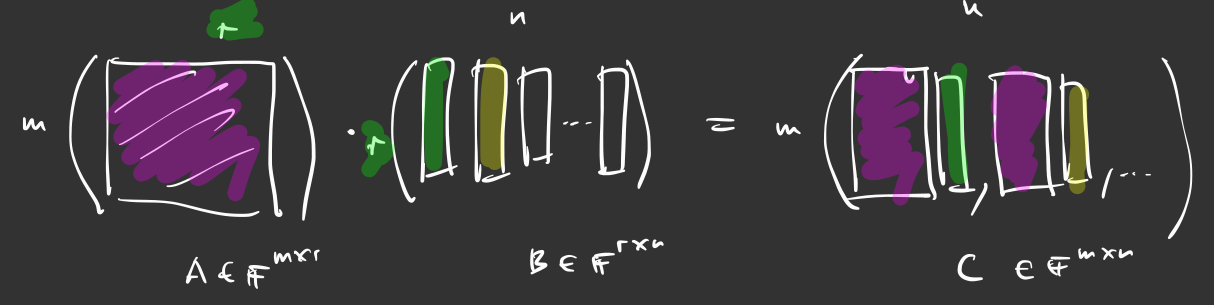
\includegraphics[height=4cm]{media/matrixmatrixproduct}~\\
}
~\\
We make this a rigorous definition:\vspace{-0.25cm}
\begin{defi}[Matrix-Matrix Product] \label{def:mat-mat-product}
	For matrices $A\in\F^{m\times r}$ and $B\in\F^{r\times n}$, we define the {\color{defgruen}\textbf{matrix-matrix product} (or simply matrix product) $C := A\cdot B \in\F^{m\times n}$} as a column wise product, i.e.,
	$$
	\begin{pmatrix}
	{\color{orange}c_{11}}&{\color[rgb]{0.1,0.5,0}c_{12}}&\ldots &{\color{cyan}c_{1n}}\\
	{\color{orange}c_{21}}&{\color[rgb]{0.1,0.5,0}c_{22}}&\ldots &{\color{cyan}c_{2n}}\\
	{\color{orange}\vdots}&{\color[rgb]{0.1,0.5,0}\vdots}&\ddots &{\color{cyan}\vdots}\\
	{\color{orange}c_{m1}}&{\color[rgb]{0.1,0.5,0}c_{m2}}&\ldots &{\color{cyan}c_{mn}}
	\end{pmatrix}
	=\begin{pmatrix}
	a_{11}&a_{12}&\ldots &a_{1r}\\
	a_{21}&a_{22}&\ldots &a_{2r}\\
	\vdots&\vdots&\ddots &\vdots\\
	a_{m1}&a_{m2}&\ldots &a_{mr}
	\end{pmatrix}
	\cdot
	\begin{pmatrix}
	{\color{orange}b_{11}}&{\color[rgb]{0.1,0.5,0}b_{12}}&\ldots &{\color{cyan}b_{1n}}\\
	{\color{orange}b_{21}}&{\color[rgb]{0.1,0.5,0}b_{22}}&\ldots &{\color{cyan}b_{2n}}\\
	{\color{orange}\vdots}&{\color[rgb]{0.1,0.5,0}\vdots}&\ddots &{\color{cyan}\vdots}\\
	{\color{orange}b_{r1}}&{\color[rgb]{0.1,0.5,0}b_{r2}}&\ldots &{\color{cyan}b_{rn}}
	\end{pmatrix}
	\,  ,\text{ i.e. }
	\begin{array}{l}
	\fbox{$\displaystyle c_{ij}=\sum\limits_{{\color{orange}\ell}=1}^ra_{i{\color{orange}\ell}}b_{{\color{orange}\ell} j}$}\\
	i=1,\ldots ,m\\
	j=1,\ldots ,n
	\end{array}
	$$
\end{defi}
\Hide{Note that it is of utmost importance that the matrix dimensions fit in so far as the middle dimension of $A\in\F^{m\times r}, B\in\F^{r\times n}$ (i.e., $r$) is the same. Otherwise, this product cannot be formulated!}
\end{frame}




%% PUT INTO EXERCISE
\begin{frame} 
\Hide{
\textbf{Question:} How do matrix sum (see Def. \ref{def:sum_scale_mats}) and matrix product (see Def. \ref{def:mat-mat-product}) get along in a mixed expression?\\~\\
We can prove the following rules:\\
\begin{lemma}[Compatibility properties of matrix sum and product] \label{lem2.4} 
Let $A,\tilde{A} \in \F^{m\times n}$, $B, \tilde{B} \in \F^{n\times 
l}$, $C \in \F^{l\times t}$, $r \in \F $. Then  
\begin{eqnarray*}
\begin{array}{lr@{~~~}l} 
	(i) & (Associativity) & (A\cdot B) \cdot C = A\cdot (B\cdot C) \hspace*{8cm} \\ 
	(ii) & \mbox{$($Distributivity}\, 1) & (A+\tilde{A})B = AB + \tilde{A} B\\ 
	(iii) & \mbox{$($Distributivity}\, 2) & A(B+\tilde{B}) = AB + A\tilde{B} \\ 
	(iv) & \mbox{(left/right neutral)} & I_m A = AI_n = A \\ 
	(v) & & (r\cdot A)\cdot B  = r(A\cdot B) = A(r\cdot B)\\ 
	(vi) & \mbox{(left/right null)} & 0A = A0 = 0 
\end{array}  \end{eqnarray*} 
\end{lemma} 
\begin{proof}
%
Only a) is not trivial:
$$
[(A\cdot B) \cdot C]_{ij} = \sum\limits_{r=1}^l\left(\sum_{k=1}^n a_{ik}b_{kr}\right)c_{rj}
=\sum_{k=1}^n a_{ik} \left(\sum\limits_{r=1}^lb_{kr}c_{rj}\right)=
[A\cdot (B \cdot C)]_{ij}.
$$  
\end{proof}
}
\end{frame}



\begin{frame}
	\textbf{The (conjugate) Transpose Matrix}\\	~\\
	We finally introduce the operation of transposing matrices (and vectors):
	\begin{defi}[Conjugate Transpose matrix]\label{def:transpose}~\\
		For a matrix $A:=(a_{ij})_{ij}\in\F^{m\times n}$ the \textbf{conjugate (or Hermitian) transpose matrix $A^H$ of $A$} is defined as
		$$A^H:=(\overline{a}_{ji})_{ij}\in\F^{n\times m},$$
		where $\overline{a}_{ji}$ denotes the complex conjugate of the coefficient $a_{ji}$. 
		~\\
		For a real matrix  $A:=(a_{ij})_{ij}\in\R^{m\times n}$, so that $\overline{a}_{ji} = a_{ji}$, this simplifies to 
		$$A^\top := A^H =(a_{ji})_{ij}\in\R^{n\times m}$$
		which we then simply call the \textbf{transpose matrix $A^\top$ of $A$}.
	\end{defi}
\Hide{
	Observe that we have the relation $$A^H = \overline{A}^T, $$
	where $\overline{A}$ is understood as the component-wise complex conjugate.
	~\\
		\begin{example}[Conjugate transpose]~\\
			\begin{itemize}
				\item Transposing a matrix.
				\item Transposing a vector.
				\item The inner product can be written as $x^H y$ (or $x^\top y$ for real vectors).
				\item Adjoint operator: Consider a matrix $A = [a_1, a_2] \in \R^{3 \times 2}$ which maps $\R^2 \to \R^3$. Then $A^\top\in \R^{2 \times 3}$ maps $\R^3 \to \R^2$ and 
				$$A^T p = \begin{pmatrix}
				a_1^\top p\\a_2^\top p
				\end{pmatrix} $$
				collects all inner products of $p$ with the columns. We will relate the inner product to projections later on.
			\end{itemize}
		\end{example}
	}
\end{frame}
 
\begin{frame}
	\Hide{Exercise:\\~\\
	 \textbf{Question:} How do transposing and other matrix operations behave in mixed expressions?\\
~\\
	We can prove the following properties
	\begin{lemma}[Rules for transposing]
		Let $A\in\mathbb{F}^{m\times r}, B\in\mathbb{F}^{r\times m}$ and $r \in \F$. Then
	\begin{enumerate}[i]
		\item[i)] Transposing twice: $(A^H)^H =A$,
		\item[ii)] Matrix product: $(AB)^H=B^H A^H$ ,
		\item[iii)] Scalar product: $(rA)^H= \overline{r} A^H$ ,
		\item[iv)] Matrix sum: $(A+B)^H= A^H + B^H$ ,
		\item[v)] Inverse (see below): For $A\in GL(n,\mathbb{F})$ we have $(A^{H})^{-1}=(A^{-1})^{H}$.
	\end{enumerate}	 
	\end{lemma}
\textbf{Remark:} For real matrices (i.e., $\F=\R$ in the lemma above), the same rules hold true for $(\cdot)^\top$.
\begin{proof}\small
	Apply definitions and exploit properties of $\F$. 
	%TODO
%	Exemplary we show
%		\begin{align*}
%		&C := A \cdot B, C := [c_{ij}]_{ij}, c_{ij} = \sum\limits_{k=1}^n a_{ik}b_{kj}, A^T = [a^\prime_{ij}]_{ij}, B^T = [b^\prime_{ij}]_{ij},\\
%		&[C]_{ij} = C_{ij} = \sum\limits_{k=1}^n a_{jk}b_{ki} = \sum\limits_{k=1}^n a^\prime_{kj}b^\prime_{ik} = \sum\limits_{k=1}^n b^\prime_{ik}a^\prime_{kj} = [B^T A^T]_{ji} \Rightarrow C^T = B^T A^T\\
%		&A \in GL(n, \mathbb{F}), A^{-1}A = I_n \;\; \Rightarrow \;\; \underbrace{(A^{-1}A)^T}_{A^T (A^{-1})^T} = I_n^T = I_n\\
%		&\Rightarrow (A^{-1})^T = (A^T)^{-1}, \text{because Inverse is unique}
%		\end{align*}
\end{proof}

}

\end{frame}

\begin{frame}
\Subsection{Span and Image -- Linear Independence and Kernel }
\Hide{
\begin{example}[Span and Image]\label{ex:span-image}~\\
\textbf{Span:}	Let us again consider the two real vectors
	$$\laVecOneSym=\laVecOneVal,~
	a_2=\begin{pmatrix}2\\0\\1\end{pmatrix}\in\mathbb{R}^3.$$
		Question: What are the vectors that we can represent as linear combination thereof?\\ 
	 There are two operations involved:~\\
	\begin{itemize}
		\item[$\cdot$:]
		Scaling each vector $a_1$ and $a_2$ individually yields infinite lines through these vectors.~\\
		\item[$+$:]
		By adding arbitrary vectors from these lines we fill out the infinite plane in-between.
	\end{itemize}
 All combinations of these two vectors form an infinite plane in $\R^3$. We say the plane is ``spanned'' by $a_1$ and $a_2$. The terminology for the set of all linear combinations is therefore accordingly:
\begin{align*}
\text{span}(a_1,a_2):=
\lbrace x_1\begin{pmatrix}1\\2\\0\end{pmatrix}
+x_2\begin{pmatrix}2\\0\\1\end{pmatrix}
:~x_1,x_2\in\mathbb{R}
\rbrace.
\end{align*}
~\\
\textbf{Image:} By considering these two vectors as columns of a matrix, more precisely,
$$
A=\begin{pmatrix}1&2\\2&0\\0&1\end{pmatrix},
$$
the analogue notion is given by the so-called \textit{image} of the matrix, which collects all matrix--vector products, i.e., 
$$\im(A)~:=\{Ax:~x\in\mathbb{R}^2\}=\lbrace x_1\begin{pmatrix}1\\2\\0\end{pmatrix}
+x_2\begin{pmatrix}2\\0\\1\end{pmatrix}
:~x_1,x_2\in\mathbb{R}\rbrace~=~\text{span}(a_1,a_2).$$
\end{example}
}
\end{frame}
%
\begin{frame}
The set of all possible linear combinations or matrix--vector products is given a special name:
\begin{definition}[Span and Image] \label{def:image-span}~\\
	\begin{itemize}
		\item[i)] The \textbf{span of \underline{vectors} $a_1, \ldots, a_n \in \F^m$} is defined by
		$$ \spann(a_1,\ldots, a_n) :=  \left\lbrace  \sum_{i=1}^n x_i a_i : x_i \in \F \right\rbrace  \subset \Fm.$$
		The set $\{a_1, \ldots, a_n\}$ is called \textbf{generating system} of $\spann(a_1,\ldots, a_n)$.~\\~\\
		\item[ii)] The \textbf{image (or column space) of a \underline{matrix} $A :=[a_1, \ldots,a_n] \in \Fmn$} is defined by
		$$ \im(A) :=  \{Ax:x\in \Fn \} = \spann(a_1,\ldots, a_n) \subset \Fm.$$
	\end{itemize}
\end{definition}
\Hide{~\\
With this terminology we find 
\begin{center}
	``$Ax = b$ is solvable''~~ $\Leftrightarrow$~~ $b$ is spanned by the columns of $A$ ~~$\Leftrightarrow$~~$b \in \im(A)$.
\end{center}
\demo{picture}\\ 
\small
Consider the example from above (i.e., $\laMatSym := [\laVecOneSym, \laVecTwoSym]$) and some vector $b=\laRHSone$. By ``solving'' the system $Ax=b$ we want to find a linear combination of the columns $a_1$ and $a_2$ (i.e., scalars $x_1$ and $x_2$), so that this combination produces the vector $b$, i.e., 
$$Ax=b ~~\Leftrightarrow~~ x_1\cdot\begin{matrix}|\\a_1\\|\end{matrix}
+x_2\cdot\begin{matrix}|\\a_2\\|\end{matrix}=b
~~\Leftrightarrow~~~~x_1\cdot\begin{pmatrix}1\\2\\0\end{pmatrix}
+x_2\cdot\begin{pmatrix}2\\0\\1\end{pmatrix}
=\begin{pmatrix}2\\1\\3\end{pmatrix}.$$
In our example we find that this $b$ is not contained in the span of the columns $a_1, a_2$ (= the infinite plane) so that our system is \textbf{not} solvable.	In particular we find $\im(A) \subsetneqq \R{^3}$ (we say $f_A$ is not ``surjective'').
}\end{frame}	


	


\begin{frame} \small
\Hide{However, what happens if we consider an additional column, e.g.,
$$
A_2 := \begin{pmatrix}
1 & 2 & 3\\ 
2& 0 &2 \\ 
0 & 1 &1
\end{pmatrix} ,~~\text{or}~~~
A_3 := \begin{pmatrix}
1 & 2 & 0\\ 
2& 0 &0 \\ 
0 & 1 &1
\end{pmatrix} .
$$
What is the difference? \\
($A_2$) \textit{Dependent columns:} \\
Here we find that the new column is a linear combination of the first two columns. More precisely,
$$ 	
1\begin{pmatrix}
	1 \\ 2 \\ 0 
\end{pmatrix}
+
1\begin{pmatrix}
	2 \\ 0  \\ 1 
\end{pmatrix} = \begin{pmatrix}
3 \\ 2 \\ 1
\end{pmatrix} \in \im(A).
$$
Therefore, no additional information added to the span: $A_2x=b$ is still not solvable. Furthermore, we easily find a linear combination of the three vectors that yield the zero vector:
$$
1\begin{pmatrix}1\\2\\0\end{pmatrix}+1\begin{pmatrix}2\\0\\1\end{pmatrix}+(-1)\begin{pmatrix}3\\2\\1\end{pmatrix}=\begin{pmatrix}0\\0\\0\end{pmatrix}.
$$
We will later pay special attention to all vectors $x$ for which $Ax = 0$ as here $x:=(1,1,-1)^\top\in~\ker(A_2)$.\\
($A_3$) \textit{Independent columns:}
$$	
x_1\begin{pmatrix}
1 \\ 2 \\ 0 
\end{pmatrix}
+
x_2\begin{pmatrix}
2 \\ 0  \\ 1 
\end{pmatrix}\neq\begin{pmatrix}
0 \\ 0 \\ 1
\end{pmatrix}
 ~~~ \text{for \bf all}~~ x_1, x_2.
$$
Thus, in this case we find
\begin{align*}
x_1\begin{pmatrix}1\\2\\0\end{pmatrix}+x_2\begin{pmatrix}2\\0\\1\end{pmatrix}+x_3\begin{pmatrix}0\\0\\1\end{pmatrix}\stackrel{!}{=}0~~~
\Rightarrow~~x_1=x_2=x_3=0
\end{align*}
We will later understand: $A_3x=b$ is definitely solvable.
}
\end{frame}


\begin{frame}
Let us properly define these concepts:
\begin{definition}[Linear independence and kernel]\label{def:linIndep_Kernel}~\\
	\begin{itemize}
		\item[i)] \underline{Vectors} $a_1, \ldots, a_r \in \F^m$	are called \textbf{linearly independent}, if the only combination that gives the zero vector is $0a_1 + \cdots+0 a_r$.\\
		%In this case, we say that $\spann(a_1,\ldots, a_r)$ has \textbf{dimension} $r$.\vspace{0.2cm}
		\item[ii)] The \textbf{kernel} of a \underline{matrix} $A \in \Fmn$ is defined by $$\ker(A) := \{x\in\Fn: Ax = 0\},$$
		i.e., the preimage of $\{0\}$ under $f_A$. 	
	\end{itemize}
\end{definition}
~\\~\\
 We find the following important equivalent formulation of linear independence:\\
  \begin{lemma} \label{lem:linear-independence}
 	For vectors $a_1,...,a_r \in \Fn$ we have the equivalence:
 	\begin{align*}
 	a_1,...,a_r~~ \text{linearly independent}
 	~~\Leftrightarrow~~
 	&\text{every vector $b \in \text{span} (a_1,...,a_r)$ can be \textbf{uniquely}}\\
 	&\text{linearly combined from the set $\{a_1,...,a_r\}$, i.e.,}\\
 	&\exists_1 x_1,\ldots,x_r \in \F\colon b = x_1a_1 + \ldots +x_ra_r.
 	\end{align*}
 \end{lemma}
 ~\\
\textit{Remark.} This result implies the following for solutions of linear systems: Let $x$ solve $Ax=b$. If $A$ has independent columns, then the solution $x$ is unique! On the contrary, if the columns are dependent, we will learn that there are infinitely many solutions!
\end{frame}

\begin{frame}
	\Hide{
	\begin{proof}[Proof of Lemma \ref{lem:linear-independence} ] 
	Strategy: We split $\mathcal{A} \Leftrightarrow \mathcal{B}$ into $\mathcal{A} \Rightarrow \mathcal{B}$ and  $\mathcal{A}\Leftarrow \mathcal{B}$.
	\begin{itemize}\blank
		\item$\mathcal{A} \Rightarrow \mathcal{B}$: Let $a_1, \cdots a_r$ be linearly independent and $b \in \spann(a_1, \cdots ,a_r)$. To show unique existence, we assume that there exist two instances and show that they are the same. Therefore, let us assume that there are two sets of coefficients, say $x_i$ and $y_i$, so that
		\begin{align*}
			b = \sum\limits_{i=1}^r x_i a_i ~~\text{and}~~ b= \sum\limits_{i=1}^r y_i a_i.
		\end{align*}
		We know that such coefficients exist, since $b \in \spann(a_1, \cdots ,a_r)$ by assumption. Now we find
		\begin{align*}
		& 0 = b-b=\sum\limits_{i=1}^r x_i a_i - \sum\limits_{i=1}^r y_i a_i = \sum\limits_{i=1}^r (x_i - y_i) a_i\\
		&\Rightarrow x_i - y_i =0,\;\text{since}\; a_1, \cdots,a_r \;\text{are linearly independent}\\[10pt]
		&\Rightarrow x_i = y_i , \;\text{i.e., linear combination is unique.}
		\end{align*}
		\item$\mathcal{A} \Leftarrow \mathcal{B}$: We apply a proof by contradiction (i.e., $\neg \mathcal{A} \Rightarrow \neg \mathcal{B} $). For this purpose, we assume $a_1, \cdots, a_r$ are linearly dependent ($\neg \mathcal{A}$), so that there exist ${x_1,\cdots, x_r \in \F}$ with $x_j \neq 0$ for at least one $x_j$, so that
		$$0= \sum\limits_{i=1}^r x_i a_i = \sum\limits_{i=1,i\neq j}^r x_i a_i + x_j a_j.$$
		Since $x_j \neq 0$, we can write $a_j = 0a_1 +\ldots+1a_j+\ldots+0a_r$ also as another linear combination 
		$$ a_j = \sum\limits_{i=1,i \neq j}^r \frac{-x_i}{x_j}a_i =  \frac{-x_1}{x_j}a_1 +\ldots +0 a_j +\ldots  +\frac{-x_r}{x_j}a_r.$$
		Thus the linear dependence ($\neg \mathcal{A}$) applies that there exists a $b \in \spann (a_1,...,a_r)$ (here $a_j$), which is not uniquely linearly combined from $a_1,\ldots, a_r$ ($\neg \mathcal{B}$).
	\end{itemize}
\end{proof}
}
\end{frame}

%\begin{frame}\tiny
%			\textit{deprecated:}\\
%			\begin{lemma} \label{lem:linear-independence}
%				For vectors $v_1,...,v_r \in V$ the following statements are equivalent: 
%				\begin{itemize} 
%					\item[(i)] The $v_1,...,v_r$ are linearly independent.
%					\item[(ii)] every vector $v \in \text{span} (v_1,...,v_r)$ can be uniquely linearly combined from the set 
%					$\{v_1,...,v_r\}$. 
%					\item[(iii)] None of $v_i$ for $ i = 1,\ldots,r$ can be written as a linear combination of the other. 
%				\end{itemize} 
%			\end{lemma}
%			Proof of Lemma \ref{lem:linear-independence}
%			\begin{proof} 
%				Strategy: show (i) $\Rightarrow$ (ii) $\Rightarrow$ (iii) $\Rightarrow$ (i)
%				\begin{itemize}\blank
%					\item[\blank a)] $(i) \Rightarrow (ii)$: $(v_1, \cdots v_r)$ linear independent, let $v \in span(v_1, \cdots ,v_r)$ be combined in two combinations: \begin{align*}
%					&r = \sum\limits_{i=1}^r \lambda_i v_i \;\text{and}\; v= \sum\limits_{i=1}^r \mu_i v_i\\
%					&\Rightarrow 0 = \sum\limits_{i=1}^r \lambda_i v_i - \sum\limits_{i=1}^r \mu_i v_i = v= \sum\limits_{i=1}^r (\lambda_i - \mu_i) v_i\\
%					&\Rightarrow \lambda_i - \mu_i =0,\;\text{since}\; v_1, \cdots,v_r \;\text{are linearly independent}\\[10pt]
%					&\Rightarrow \lambda_i = \mu_i , \;\text{i.e. linear combination is unique}
%					\end{align*}
%					\item[\blank b)] $(ii) \Rightarrow (iii)$: \text{proof by contradiction: assume we have} $a_{ij}$ \text{with} $v_j = \sum\limits_{i=1, i \neq j}^r v_i$\vspace{-0.2cm}
%					\begin{align*}
%					&\text{take}\; \lambda_j := -1 \Rightarrow 0 = \sum\limits_{i=1}^r \lambda_i v_i \;\text{with} \; \lambda_j = -1\\
%					&\text{but also}\; 0 = \sum\limits_{i=1}^r 0\cdot v_i\\
%					&\Rightarrow \;\text{has two different representations as linear combinations of}\; \{v_1,\cdots,v_r\}\hspace{1cm} \lightning (ii)
%					\end{align*} 
%					\item[\blank c)] $(iii) \Rightarrow (i)$: proof by contradiction: assume $v_1, \cdots, v_r$ are linear independent $\Rightarrow \exists{\lambda_i,\cdots, \lambda_r \in \mathbb{F}}$ with $\lambda_j \neq 0$ for at least one $\lambda_j$ with:
%					\begin{align*}
%					&0= \sum\limits_{i=1}^r \lambda_i v_i = \sum\limits_{i=1,i\neq j}^r \lambda_i v_i + \lambda_j v_j\\
%					&\Rightarrow v_j = \sum\limits_{i=1,i \neq j}^r (\frac{-\lambda_i}{\lambda_j})v_i \hspace{1cm} \lightning (iii)
%					\end{align*}
%				\end{itemize}
%			\end{proof}
%		\end{frame}



% SUMMARY
\begin{frame}
	\Hide{
\textbf{Summary:} Relation between vector and matrix notions\\
~\\
	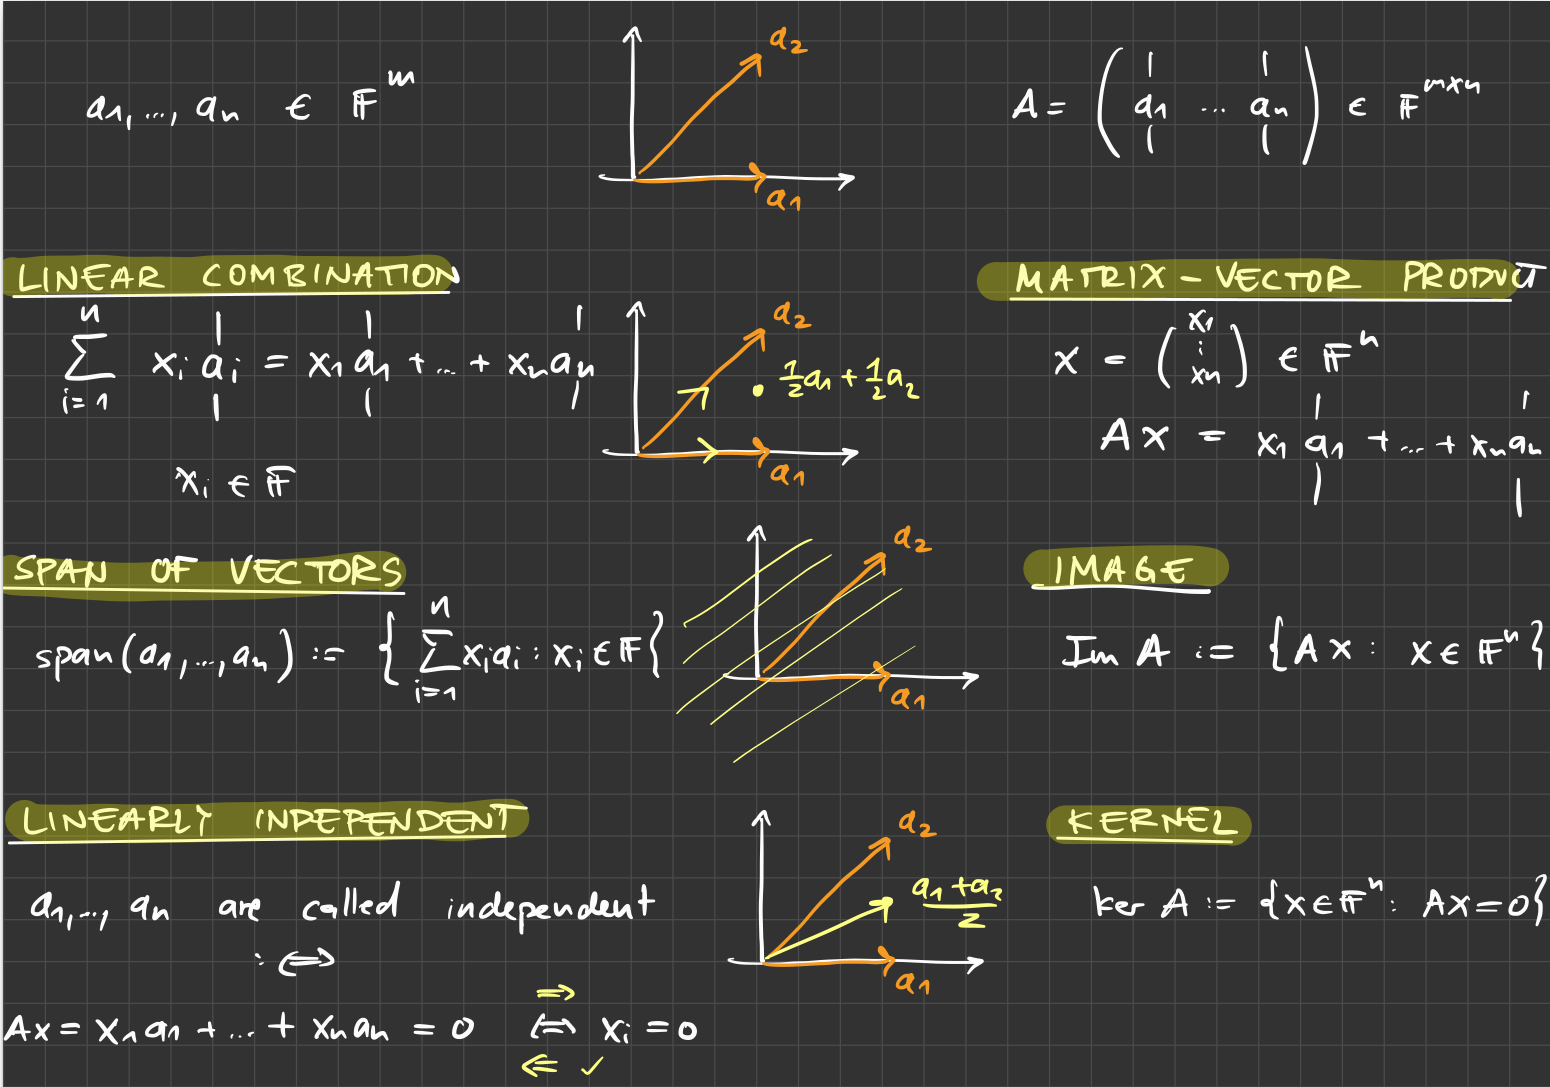
\includegraphics[width=0.9\linewidth]{media/vectorVSmatrix}
}
\end{frame}






%======================
\begin{frame}
\Subsection{Subspaces of $\F^n$ -- Basis and Dimension}
\Hide{
\begin{example}[Subspaces]~\\
	Let $\F = \R$.
	\begin{itemize}
	\item $n=2$: A straight line $L:= \{x a\colon x \in \R\}\subset\R^2$ spanned by a fixed $a\in\R^2$. For a linear function $f(x)=mx$ with $m:=\tfrac{a_2}{a_1}$ we find 
	$$\text{graph}(f)
	:=\{(x,f(x)): x \in \R\} 
	=\{(x,mx): x \in \R\} 
	= \spann(\begin{pmatrix}
	1\\
	\tfrac{a_2}{a_1}
	\end{pmatrix})
	= \spann(\begin{pmatrix}
	  a_1\\
    a_2
	\end{pmatrix})~~~(\text{note:}~ a_1\R = \R) 
	$$
		\item  $n=3$: A plane $P:= \{x_1 a_1+ x_2 a_2\colon x_i \in \R\}\subset \R^3$ spanned by fixed $a_1, a_2\in\R^3$.\\
	\item  Not a (linear) subspace: The graph of nonlinear functions, such as $x^2$ or $\sin(x)$ in $\R^2$.
\end{itemize}
\demo{pictures}
\end{example}
~\\~\\
}

%
\begin{definition}[Subspace] \label{def:subspace}
	A subset $V \subset \F^n$ is called \textbf{(linear) subspace of $\F^n$} if 
	\begin{itemize}
		\item[i)] it is nonempty, i.e., $V\neq \emptyset$,
		\item[ii)] and if it is closed under linear combinations, i.e., if 
		\begin{align*}
		\lambda_1 v_1 + \lambda_2 v_2 \in V ~~~\text{for all}~~~v_1, v_2 \in V,~\lambda_1, \lambda_2 \in \F .
		\end{align*}
	\end{itemize} 
\end{definition}
\end{frame}




\begin{frame}
\textbf{Question:} Is it possible to describe a linear subspace of $\Fn$ by a finite number of vectors?
\begin{definition}[Basis]\label{def:basis}
Let $V \subset \F^n$ be a subspace of $\F^n$. Then a set of vectors $\{v_1, \ldots, v_r\} \subset V$ with $r\leq n$ is called \textbf{basis of $V$}, if 
\begin{itemize}
	\item[i)] $v_1, \ldots, v_r$ are linearly independent,
	\item[ii)] $\text{span}(v_1, \ldots, v_r) = V$.
\end{itemize}
\end{definition}
~\\
\Hide{
		\begin{itemize}\blank
	\item Let $\{v_1, \ldots, v_r\} \subset V$ be a basis. Then, in particular, any $v \in V=\text{span}(v_1, \ldots, v_r)$ can be written as
	\begin{align*}
	v = \sum_{j=1}^r \lambda_j v_j
	\end{align*}
	for some \textit{uniquely} determined scalars $\lambda_j \in \F $ (see Lemma \ref{lem:linear-independence}).\\
	$\rightarrow$ These scalars are called \textbf{\color{defgruen} coordinates} of $v$ with respect to the basis $\{v_1, \ldots, v_r\}$. ~\\~\\
	\item One can show that 
	\begin{itemize} \normalsize
		\item {\color{satzrot}there exists a basis} (general result based on Zorn's lemma),
		\item {\color{satzrot}any basis of a subspace of $\F^n$ has the same length} (doable proof), which we call \textbf{\color{defgruen}dimension of $V$ ($\dim(V)$)}.
	\end{itemize} 
~\\
	\item With other words: 
	\begin{center}
		\textit{The maximum number of linearly independent vectors is called dimension and the set of such vectors is called a basis.}
	\end{center}
\end{itemize}
}
\end{frame}


%%
\begin{frame}
\Hide{ \small
\begin{example} \label{ex:subspaces}
~\\
\textbf{1)} Let us consider $\F =  \R$ and $V:= \mathbb{R}^2\subset \R^2$.\\~\\
We first show that $V$ is a subspace of $\mathbb{R}^2$ and then try to find some bases.~\\
Following Definition \ref{def:subspace} we show:\\
\begin{itemize}
	\item[i)] $V \neq \emptyset$: Consider $0 \in V$.
	\item[ii)] $V$ is closed under linear combinations: Let $v_1, v_2 \in V,~\lambda_1,\lambda_2 \in \R$, then clearly $\lambda_1v_1+\lambda_2v_2 \in \R^2=V$.
\end{itemize}
Now it makes sense to talk about a \textit{basis} for $V$. We next try to find a set of vectors $v_1,\ldots, v_r \in V$ that satisfies Definition \ref{def:basis}.\\

\begin{itemize}
	\item[\textbf{1a)}] Let us consider the vectors $e_j := (\delta_{ij})_{1\leq i \leq n} = (0\ldots 1 \ldots 0)^\top \in \Rn$, here with $n=2$. We show that $\{e_1,e_2\}$ is a basis of $V$ by verifying the two conditions in Definition \ref{def:basis}.
	\begin{itemize}
		\item[i)] We show that $e_1,e_2$ are linearly independent. From
		$$x_1e_1+x_2e_2=\begin{pmatrix}x_1\\x_2\end{pmatrix}\stackrel{!}{=}0$$	
		we easily conclude that $x_1=0=x_2$, so that $e_1,e_2$ are indeed linearly independent.
		\item[ii)] By Definition \ref{def:sum_scale_mats} any $v=\begin{pmatrix}v_1\\v_2\end{pmatrix}\in V=\mathbb{R}^2$ can be written as
		$$v=v_1\begin{pmatrix}1\\0\end{pmatrix}+v_2\begin{pmatrix}0\\1\end{pmatrix} = v_1e_1+v_2e_2.$$
		Thus 
		$$V = \R^2 = \{v_1e_1+v_2e_2 \colon v_1,v_2 \in \R \} =\text{span}(e_1,e_2).$$
	\end{itemize}
In terms of the previous slide, we have that	$v_1,v_2$ are the coordinates of $v$ w.r.t the basis $\{e_1,e_2\}$ and the dimension of $V$ is 2, we write $\dim(V)=2$.\\~\\
	\textit{\textbf{Remark}: Analogue results hold true for any $\R^n$ (not just $n=2$) and the set of vectors $\{e_1,\ldots,e_n\}$ is called the {\color{defgruen}standard basis} or {\color{defgruen}unit vectors in $\Rn$}.}
\end{itemize}
\end{example}
}
\end{frame}

%%
\begin{frame}
	\Hide{\footnotesize 
	\begin{itemize}
		\item[\textbf{1b)}] Let us find another basis for $\R^2$ and check whether its length is still 2 in accordance with the remarks after Definition \ref{def:basis}.\\
		For instance, let us consider the vectors
	$$a_1=\begin{pmatrix}1\\0\end{pmatrix},~a_2=\begin{pmatrix}1\\1\end{pmatrix} \in V.$$
Again, we verify that the two conditions in Definition \ref{def:basis} are satisfied:
\begin{itemize}\footnotesize
	\item[i)] Now let us use the equivalent formulation of linear independence from Lemma \ref{lem:linear-independence}. For this purpose let $v \in \text{span}(a_1,a_2)$ so that there exist scalars $\lambda_1,\lambda_2\in\mathbb{R}$ with
	$$\begin{pmatrix}v_1\\v_2\end{pmatrix} = \lambda_1a_1+\lambda_2a_2,$$
	which, after inserting the precise numbers for $a_1$ and $a_2$, is equivalent to
	$$\begin{pmatrix}\lambda_1\\0\end{pmatrix}
	+\begin{pmatrix}\lambda_2\\\lambda_2\end{pmatrix}
	=\begin{pmatrix}v_1\\v_2\end{pmatrix}.$$
	Using matrix notation we can even write
	$$\begin{pmatrix}
	1&1\\0&1
	\end{pmatrix}\cdot \begin{pmatrix}\lambda_1\\\lambda_2\end{pmatrix} = \begin{pmatrix}v_1\\v_2\end{pmatrix}. $$
	In order to apply Lemma \ref{lem:linear-independence}, we need to show that the scalars $\lambda_1,\lambda_2$ are uniquely determined by this equation. Therefore, let us now solve this upper triangular system (we will later learn about \textit{backward substitution} to do this algorithmically). We observe from the bottom equation that
	$\lambda_2=v_2. $
	Inserting this into the top equation then yields
	$$\lambda_1+\lambda_2=v_1 ~~\Leftrightarrow~~\lambda_1+v_2=v_1~~\Leftrightarrow~~\lambda_1=v_1-v_2.$$
	Observe that $\lambda_1$ and $\lambda_2$ are uniquely determined, i.e., there are no other $\lambda_1$ and $\lambda_2$ solving the upper equations; thus $a_1,a_2$ are independent by Lemma \ref{lem:linear-independence}. Also, let us make a quick test:
	$$(v_1-v_2)a_1+v_2a_2 =\begin{pmatrix}v_1-v_2\\0\end{pmatrix}+\begin{pmatrix}v_2\\v_2\end{pmatrix}
	=\begin{pmatrix}v_1\\v_2\end{pmatrix}. $$
	\item[ii)] We note that $\text{span}(a_1,a_2) \subset \R^2 = V$ is obviously true and to prove the reverse subset relation we choose the scalars $\lambda_1=v_1-v_2,~\lambda_2=v_2$ for $v=(v_1,v_2)^\top \in V=\R^2$.
\end{itemize}
		All in all, we have that $\lambda_1=v_1-v_2,~\lambda_2=v_2$ are the coordinates of $v \in V$ w.r.t the basis $\{a_1,a_2\}$ of $V$ and $\dim(V)=2$. \\
		\Vspace{0.1cm}
		\textit{\textbf{Remark:} The notation for vectors introduced in D. \ref{def:matrix} implicitly assumes that vectors are represented in the standard basis.} 
	\end{itemize}
}
\end{frame}



%
%\begin{frame}
%\begin{theorem}\label{basis-complement} Let $V$ be a vector space over the field $\F $. 
%\ite
%\item[i)] if $V=\text{span}(v_1,\ldots,v_n)$, then any linearly independent set $\{w_1,\ldots,w_r\}\subset V$ ($r<n$), can be complemented by elements from $\{v_1,\ldots,v_n\}$ to a basis of $V$.
%\item[ii)] if $V$ has a finite basis ($n < \infty$), then any basis has the same length, which we call \emph{\color{defgruen} \textbf{dimension}} of $V$.
%\item[iii)] a set $\{v^1,\ldots ,v^n\}\subset \F^n$ is a basis of  
%$\F^n$, if the matrix consisting of these vectors as columns
%\[
%A:=\left[\begin{array}{c@{\quad}c@{\quad}c@{\quad}c}
%v^1 & v^2 & \dots & v^n
%\end{array}\right]
%:=
%\left[\begin{array}{cccc}
%v^1_1 & v^2_1 & \dots & v^n_1\\
%v^1_2 & v^2_2 & \dots & v^n_2\\
%\vdots & \vdots & \dots & \vdots\\
%v^1_n & v^2_n & \dots & v^n_n
%\end{array}\right]
%\]
%is invertible.
%\eti 
%\end{theorem}
%\end{frame}





\begin{frame}
In the exercises we will prove that for any matrix $A \in \Fmn$, the kernel $\ker(A)$ is a subspace of $\Fn$ and the image $\im(A)$ is a subspace of $\Fm$. In the context of matrices these are important spaces and we give their dimensions a special name:\\
\begin{defi}[rank and nullity]\label{def:rank-nullity}
	 Let $A \in \Fmn$. Then
	\begin{itemize}
		\item[-] $\rank(A)  := \dim(\im(A))$ is called the (column) \textbf{rank of $A$},
		\item[-] $\nullity(A) := \dim(\ker(A))$ is called the \textbf{nullity of $A$}.
	\end{itemize}
\end{defi}
\Hide{~\\
\begin{example}\small~\\
	\begin{itemize}
		\item [\textbf{1)}] Let us consider the matrix $A=[a_1,a_2,a_3]:=\begin{pmatrix}
		1&1&2\\0&1&1
		\end{pmatrix} $.\\
		\textbf{1a)} By Definition \ref{def:image-span} of the image we have 
		$\im(A)=\text{span}(a_1,a_2,a_3).$
		By observing $a_3 = a_2 + a_1$, i.e., $a_3$ is a linear combination of $a_1$ and  $a_2$, we even find that $\im(A)~=~\text{span}(a_1,a_2).$
		Since the vectors $a_1, a_2$ have been identified to be linearly independent (see Example \ref{ex:subspaces}), we find by Definition \ref{def:basis} that they form a basis for $\im(A)$. Thus
		$$\rank(A) =  \dim(\im(A))=2.$$
		\textbf{1b)} What about the nullity? We first need to find a basis of the kernel (we will do this by re-writing it as a span of some independent vectors). For this purpose, let $x \in \ker(A)$, which by Definition \ref{def:linIndep_Kernel} is equivalent to
		$$Ax = 0 ~~\Leftrightarrow~~x_1+x_2+2x_3 = 0, ~~x_2+x_3 =0. $$
		Now from the second equation we obtain $x_2 = -x_3$. Let us also write $x_1$ as a function of $x_3$. This is achieved by inserting $x_2 = -x_3$ into the first equation to obtain 
		$$x_1+x_2+2x_3 =x_1-x_3+2x_3  =x_1+x_3=  0 ~~\Leftrightarrow~~x_1 = -x_3.$$
		Thus we find
		$$Ax = 0 ~~\Leftrightarrow~~x = \begin{pmatrix}
		x_1\\x_2\\x_3
		\end{pmatrix}  = \begin{pmatrix}
		-x_3\\-x_3\\x_3
		\end{pmatrix} = x_3\begin{pmatrix}
		-1\\-1\\1
		\end{pmatrix}.$$
	
	\end{itemize}
\end{example}
}
\end{frame}

\begin{frame}
	\Hide{	~\\
\begin{itemize}
	\item[] 		\small	With other words, we can write
		$$\ker(A) = \{\begin{pmatrix}
		x_1\\x_2\\x_3
		\end{pmatrix}\in\R^3\colon x = x_3\begin{pmatrix}
		-1\\-1\\1
		\end{pmatrix} \} = \{x_3\cdot\begin{pmatrix}
		-1\\-1\\1
		\end{pmatrix}\colon x_3 \in \R \} = \text{span}(\begin{pmatrix}
		-1\\-1\\1
		\end{pmatrix}).$$
		Since $\begin{pmatrix}
		-1\\-1\\1
		\end{pmatrix} \neq 0$ it forms an independent set of length 1 so that by Definitions \ref{def:basis} and \ref{def:rank-nullity} we finally conclude that 
		$$\nullity(A) = \dim(\ker(A)) =1. $$
	~\\~\\
	\textit{\textbf{Remark:} We observe that $$\rank(A) + \nullity(A) = 3~~~ \text{(=column dimension)}.$$ We will see below that this is generally true -- called the \textit{dimension formula}!}
\end{itemize}
}
	
\end{frame}


\begin{frame}
\Hide{\small	\begin{itemize}
			\item [\textbf{2)}]	Let us consider $A= [a_1,a_2]:=\begin{pmatrix}
	1&2\\1&2\\0&0
	\end{pmatrix}$.~\\ 
	\textbf{2a)} Since $a_2 = 2\cdot a_1$, the columns are certainly linearly dependent (e.g., $2\cdot a_1+ (-1)a_2 = 0 \in \R^2 $; a combination that yields zero but with nonzero coefficients). Therefore
	$$\im(A) = \text{span}(a_1, a_2) = \text{span}(a_1), $$
	so that $$ \rank(A)=\dim(\im(A)) = 1.$$\\~\\
	\textbf{2b)} Now let us consider the kernel ker$(A) =\{x:~Ax=0\}$. Following along the lines of the previous slides we get
	\begin{align*}
	Ax=0~~&\Leftrightarrow~~\begin{pmatrix}1\\1\\0\end{pmatrix}x_1+\begin{pmatrix}2\\2\\0\end{pmatrix}x_2=\begin{pmatrix}0\\0\\0\end{pmatrix}~~
	\Leftrightarrow~~\begin{pmatrix}x_1+2x_2\\x_1+2x_2\\0\end{pmatrix}=\begin{pmatrix}0\\0\\0\end{pmatrix}
	\Leftrightarrow~~x_1=-2x_2
	\end{align*}
	and thus
	$$	\ker(A)=\{x\in\mathbb{R}^2:~x_1=-2x_2\}
	=\lbrace\begin{pmatrix}-2x_2\\x_2\end{pmatrix}\in\mathbb{R}^2:~x_2\in\mathbb{R}\rbrace
	=\lbrace x_2\begin{pmatrix}-2\\1\end{pmatrix}\in\mathbb{R}^2:~\lambda\in\mathbb{R}\rbrace
	=~\text{span}\left(\begin{pmatrix}-2\\1\end{pmatrix}\right).
$$
So all in all, $\nullity(A) = \dim(\ker(A))  =1$.\\
~\\
\textit{\textbf{Remark:} Again we observe that $$\rank(A) + \nullity(A) = 2~~~ \text{(=column dimension)}.$$}
	\item[\textbf{3)}] Similarly, considering the matrices from above we find $\rank(A_2) = 2$ and  $\rank(A_3) = 3$.
\end{itemize}}
\end{frame}

\begin{frame}

\textbf{Question:} Can we find a general relation between the nullity and the rank of a matrix?

\begin{theorem}[Dimension Formula/Rank--Nullity Theorem] \label{dimension-formula}
	Let $A \in \Fmn$, then 
$$\rank(A) +  \nullity(A) = n. $$
\end{theorem}
\Hide{
~\\
\begin{itemize}
	\item The dimension formula also reads as
$$\dm(\im(A)) + \dm(\kernel(A)) = \dm(\Fn). $$
~\\
\item \textbf{Intuition:}  Let us again think of a matrix $A \in \Fmn$ as a mapping from $\Fn$ to $\Fm$. If the matrix maps some vectors of this $n$--dimensional space $\Fn$ to $0$ -- precisely those vectors from the kernel of A -- then we can say that this ``piece of information'' gets lost. What prevails from $\Fn$ makes up the image of $A$ whose dimension is the rank of the matrix by definition. So, the amount of information in $\Fn$ equals the information that gets lost after mapping it by $A$ ($\nullity(A)$) plus the one that prevails ($\rank(A)$).
~\\
%\item We will later learn about an equivalent rank definition. More precisely, we will find that:\\~\\ \centering
%	{\color{satzrot} rank($A$) = maximum number of linearly independent column vectors.}
\end{itemize}	
}
\end{frame}



\begin{frame}\Subsection{Inverse Matrices}
	\Hide{
\begin{example}[Inverses]\label{ex:inverse}%\small
	Let us consider the following matrix
		$$A=[a_1,a_2]=\begin{pmatrix}1&1\\0&1\end{pmatrix},$$
	which is composed of the vectors considered in Example \ref{ex:subspaces} 1b).\\~\\
	\textit{Recall results Ex.\ref{ex:subspaces} 1b):} We have already observed that $a_1,a_2$ are independent and $\spann(a_1,a_2) = \R^2$. With other words, for any $b\in \R^2$, by Lemma \ref{lem:linear-independence} there exist unique (!) scalars $x_1,x_2$, so that $Ax =x_1 a_1 + x_2a_2=b$. More precisely, for $x_b=\begin{pmatrix}b_1-b_2\\b_2\end{pmatrix}$ (coordinates of $b$ wrt. the basis $\{a_1,a_2\}$) we found
	$$Ax_b=\begin{pmatrix}1&1\\0&1\end{pmatrix}
	\begin{pmatrix}b_1-b_2\\b_2\end{pmatrix}=\begin{pmatrix}b_1\\b_2\end{pmatrix}=b.$$\\~\\
	Clearly, the vector $x_b$ is composed of information from $b$.
	Now let us consider the following mapping
	$$b\mapsto x_b=\begin{pmatrix}b_1-b_2\\b_2\end{pmatrix}=
	\begin{pmatrix}	1\\0\end{pmatrix}b_1 + \begin{pmatrix}	-1\\1\end{pmatrix}b_2
	=\underbrace{\begin{pmatrix}1&-1\\0&1\end{pmatrix}}_{=:A^{-1}}\begin{pmatrix}b_1\\b_2\end{pmatrix}.$$
	We observe that the mapping from the vector $b$ to its coordinates $x_b$ w.r.t. the basis $\{a_1,a_2\}$ can be expressed as a matrix--vector product. The involved matrix $A^{-1}$ is referred to as the \textit{inverse matrix} of $A$.
\end{example}
}
\end{frame}

\begin{frame}
	\textbf{In general:}\\~\\
	Consider the matrix as a mapping $$f_A:\mathbb{F}^n\rightarrow\mathbb{F}^n,~x\mapsto Ax.$$
	Then by definition the \textit{mapping} $f_A$ is \textbf{\color{defgruen}invertible}, if there exists a mapping $f_A^{-1}:\mathbb{F}^n\rightarrow\mathbb{F}^n$ such that for all $x,b \in \mathbb{F}^n$
	we have 
	$$f_A(x)=b~~~\Leftrightarrow~~~x=f_{A}^{-1}(b).$$
	Inserting the definition of $f_A$ this reads as
	$$Ax=b~~\Leftrightarrow~~x=A^{-1}b.$$
	Verifying this condition for all possible $x$ and $b$ would be an ambitious endeavor. Luckily, this condition can be rephrased into conditions solely involving the matrix $A$. More precisely, by inserting one into the other we obtain
	\Hide{~\\
	\begin{itemize}
		\item[i)] $Ax = b  ~~\Leftrightarrow~~ AA^{-1}b=b~~\Leftrightarrow~~AA^{-1}= I $,
		\item[ii)] $x=A^{-1}b  ~~\Leftrightarrow~~ x=A^{-1}Ax ~~\Leftrightarrow~~A^{-1}A= I $.
	\end{itemize} 
~\\
	Let us quickly check this for Example \ref{ex:inverse}:\\
	 ~\\
	 $~~A^{-1}A =\begin{pmatrix}1&-1\\0&1\end{pmatrix}\begin{pmatrix}1&1\\0&1\end{pmatrix}=\begin{pmatrix}1&0\\0&1\end{pmatrix}=I_2 ~~\checkmark$,
	 ~~~  $~~AA^{-1} =\begin{pmatrix}1&1\\0&1\end{pmatrix}\begin{pmatrix}1&-1\\0&1\end{pmatrix}=\begin{pmatrix}1&0\\0&1\end{pmatrix}=I_2~~\checkmark.$


}
\end{frame}



\begin{frame} 
	Let us make this a definition.
	\vspace{0.25cm}
	\begin{defi}[Inverse matrix] \label{def2.5} 
		A matrix $A \in \F^{n\times n}$ is called {\bf invertible}, if there exists 
		a matrix $\tilde{A} \in \F^{n\times n}$ with 
		\begin{equation} \label{eq:definvertible_mat}
		A\cdot\tilde{A}  = \tilde{A}\cdot A=
		I_n.
		\end{equation}
		In case of existence we find that $\tilde{A}$ is unique (see below) and we denote by $A^{-1}:= \tilde{A}$ the {\bf inverse matrix} 
		of $A$. The set of all invertible matrices in $\Fnn$ is denoted by $GL_n (\F )$, the so-called {\em
			general linear group}.   
	\end{defi}
\Hide{
	\vspace{1.25cm}
	Consider the linear equation 
	$$Ax = b$$
	By setting $\color{cyan}x := A^{-1}b$, we find
	$$A {\color{cyan}x} = A {\color{cyan} A^{-1}b} = {\color{red} A A^{-1}}b = {\color{red}I_n}b = b .$$
	~\\
	If $A$ is invertible, then 
	\begin{center}
		``solving $Ax = b$''~~~$=$~~~``{\color{cyan} applying} the {\color{orange} inverse matrix $A^{-1}$}''\\\vspace{0.3cm}
		\hspace{3cm}{\color{cyan} (\textit{numerical methods})}  ~~~~~~~~~~~{\color{orange} (\textit{not accessible in practice})}
	\end{center}
}
\end{frame}






\begin{frame}
	From the dimension formula \ref{dimension-formula} for $n=m$, we find \textbf{``injectivity $=$ surjectivity''}\\~\\
	\Hide{	\pictures{~\\
			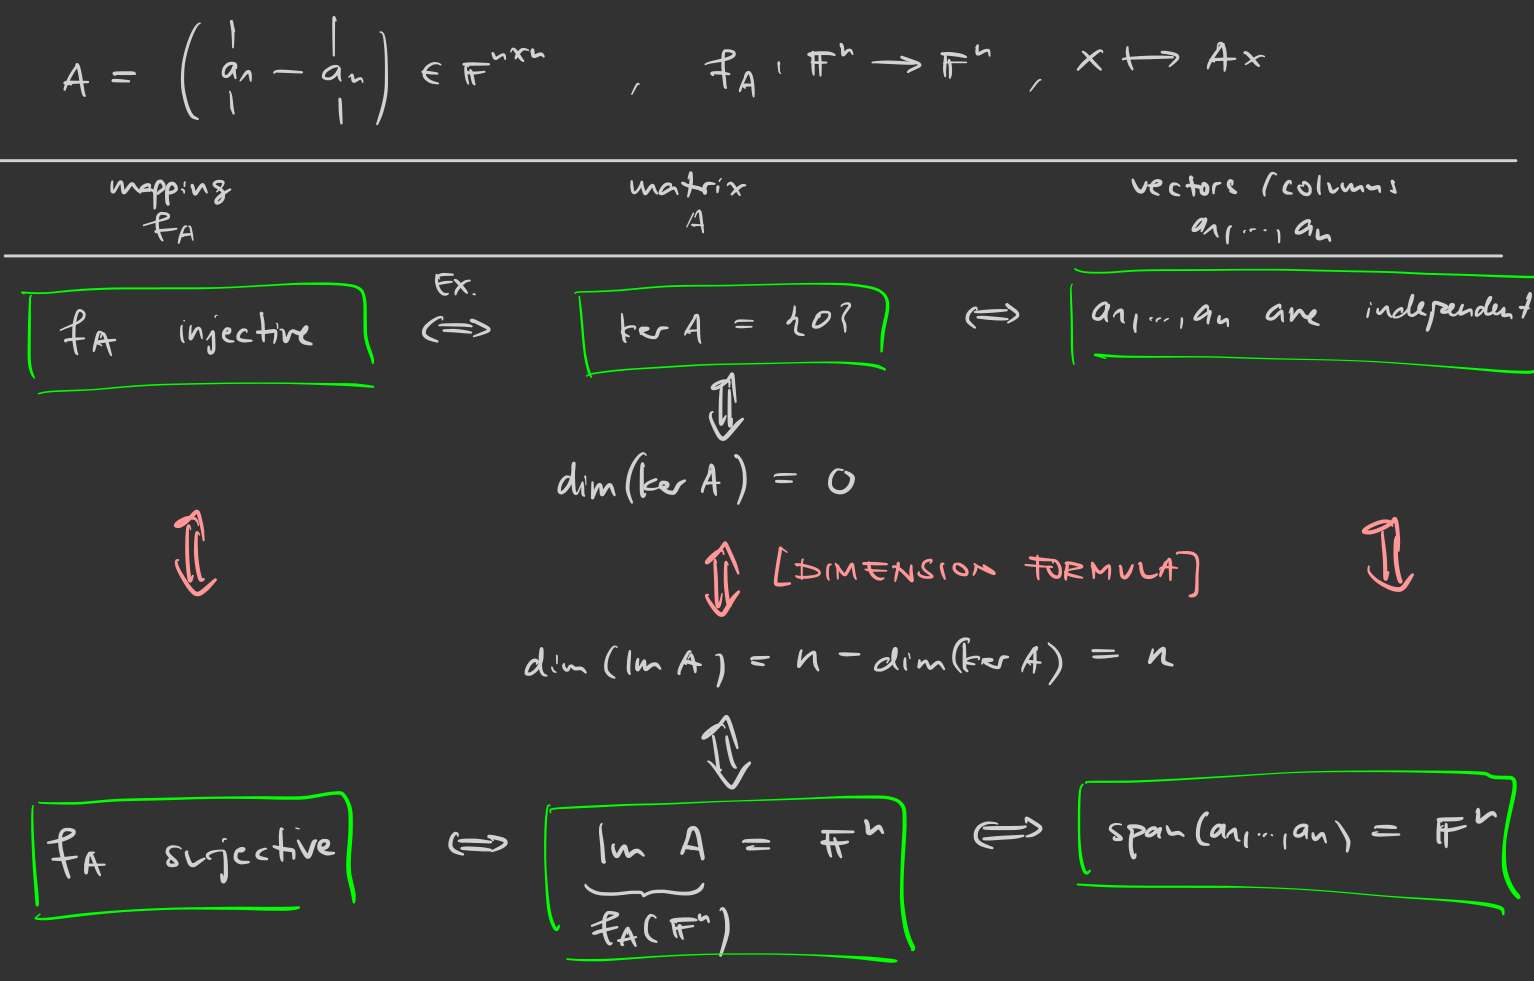
\includegraphics[width=0.9\textwidth]{media/la-InverseMatrices1}}~\\
		~\\Also see Lemma \ref{lem:linear-independence}}
\end{frame}


\begin{frame}
	\textbf{Remark:}\\ A System $Ax = b$ can be solvable even if $A$ is not squared (and thus not invertible)! \\	
~\\
\Hide{\pictures{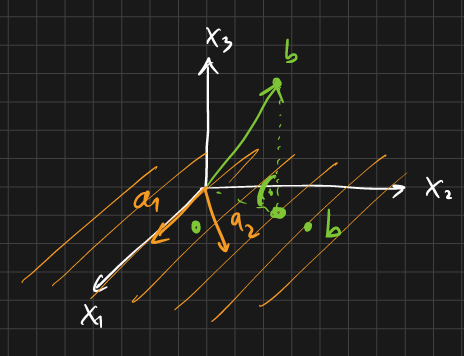
\includegraphics[width=0.17\textwidth]{media/dim-formel}}
	~\\
	The Difference:\vspace{0.2cm}
	\begin{itemize}
				\item \textit{invertible} ($m = n$): For \textbf{any} $b$ there is a \textbf{unique} $x$ so that $Ax = b$, i.e.,\\\vspace{0.2cm} 	
		~~~~~~~~~~~~~~~~~~~~~~~~~~~~~ $A$ is invertible ~~$\Rightarrow$~~ we always have that $b \in \im(A)$\\\vspace{0.2cm}
		\Hide{\textit{This unique $x$ is given by $A^{-1}b$.}\vspace{0.6cm}}
		\item \textit{solvable} ($m \neq n$ allowable): Given a \textbf{fixed} $b$ we find \textbf{at least one} $x$ so that $Ax = b$, i.e.,\\\vspace{0.2cm}
		~~~~~~~~~~~~~~~~~~~~~~~~~~~~~ $Ax=b$ is solvable ~~$\Leftrightarrow$~~ $b\in \im(A)$\\\vspace{0.2cm}
		\Hide{\textit{We will learn later that in some cases this $x$ is given by $(A^\top A)^{-1} A^\top b$.}\vspace{0.5cm}}

	\end{itemize}
~\\
	Thus:\begin{center}
		invertible~~ $\Rightarrow$~~ solvable
	\end{center} 
}
\end{frame}

\begin{frame}
	\Hide{Exercise:\\
		\begin{lemma}[Porperties of inverse matrices] \label{lem:properties-inverses}
We find the following properties:
\begin{itemize} 
			%
			\item[i)] The inverse $A^{-1}$ is also invertible, with inverse $\left(A^{-1}\right)^{-1} = A$.
			%
			\item[ii)] Since $\F$ is a field, any left-inverse is also a right-inverse and vice-versa.
			%
			\item[iii)]  An invertible matrix $A\in\Fnn$ has exactly one inverse matrix.\\
			\item[iv)] The product of two invertible matrices, say $A$ and $B$, is invertible with inverse
			$$(AB)^{-1} = B^{-1}  A^{-1} . $$
			%%
			\item[v)] A diagonal matrix 
			$$D = \text{diag}(d_1, \ldots, d_n)= \begin{pmatrix}
			d_1 & & \\
			&\ddots&\\
			&&d_n
			\end{pmatrix}\in\Fnn$$ is invertible if and only if $d_i \neq 0$ for all $i=1,\ldots, n$. Its inverse is given by $$D^{-1} = \text{diag}(d_1^{-1}, \ldots, d_n^{-1}) = \begin{pmatrix}
			d_1^{-1} & & \\
			&\ddots&\\
			&&d_n^{-1}
			\end{pmatrix}\in\Fnn.$$
\end{itemize}
		\end{lemma}
~\\
In particular, $(GL_n (\F ),\cdot)$ is a group.
	}
\end{frame}


%TODO
%ADD PROOF
%\begin{frame}
%\Hide{		\begin{proof}[Proof of Lemma \ref{lem:properties-inverses}]
%		~\\
%		\begin{itemize}
%			\item[i)] 
%			\item[ii)] Since $(A^{-1})^{-1}=A$ we find
%			\[
%			A \cdot A^{-1}=(A^{-1})^{-1}  \cdot A^{-1}=I_n
%			\]	
%			\item[iii)] Suppose $BA = I_n$ and $AC = I_n$, then
%			$$B = BI_n =B(AC) = (BA)C=I_nC = C. $$
%			\item[iv)] 		$(B^{-1} A^{-1})(AB) = B^{-1} (A^{-1}A)B = B^{-1}I_nB = 
%			B^{-1}B= I_n  $
%			\item[v)] 
%		\end{itemize}
%	
%	\end{proof}
%}
%\end{frame}






% STANDARD SCALAR PRODUCT AND 2-NORM
%\lecture{Fundamentals of Linear Algebra III}{la-3}
\begin{frame} 
\Subsection{The Euclidean Norm}
Let us first consider the 2d and 3d case:\\
\Hide{
~\\
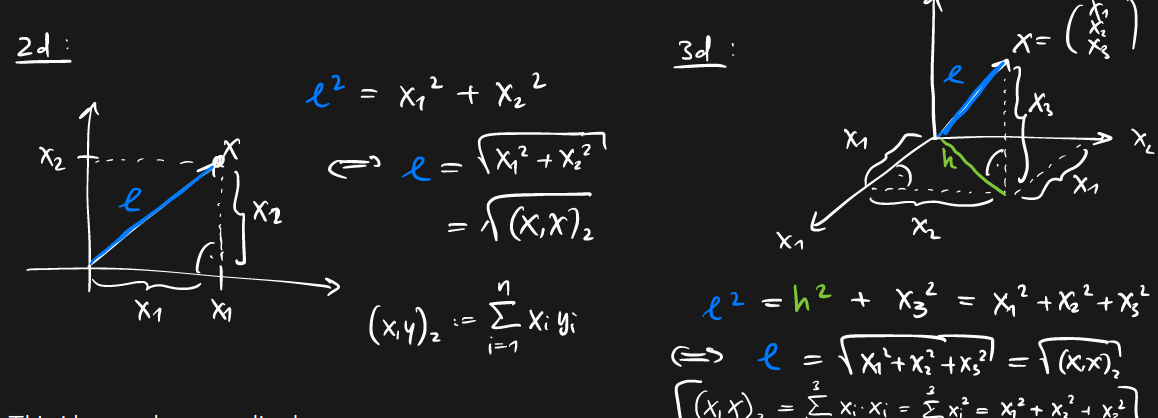
\includegraphics[width=1\textwidth]{media/pythagoras}
~\\}

This idea can be generalized to: \vspace{-0.25cm}
\begin{defi}[Euclidean Norm] 
	The Euclidean norm of a vector $x\in \F^n$ is defined by $$\|x\|_2 := \sqrt{\sum_{i=1}^n |x_i|^2}= \sqrt{x^H x} $$
	where $|a+ib|^2 := a^2+b^2$ denotes the absolute value of a complex number.
	For a real vector $x\in \R^n$ this simplifies to
	$\|x\|_2 := \sqrt{\sum_{i=1}^n x_i^2}= \sqrt{x^\top x}. $
\end{defi}
\small
{ $\rightarrow$ We will also get to know other ``norms'' (e.g., Manhattan norm or maximum norm).}\\


\end{frame}
\begin{frame} 
	\textbf{Relating the inner product to \text{projections}}~\\\vspace{0.2cm}
	Let us consider $\F=\R$. As a special case of the so-called \textbf{Cauchy Schwarz inequality} one can show that, for any two real vectors $x,y\in \R^n$, 
	\begin{equation*}\label{eq:cauchyschwarz_l2} \color{satzrot}
	\left|x^Ty\right|\le \|x\|_2\cdot\|y\|_2.
	\end{equation*}
	~\\
	This is equivalent to (assumed both vectors are nonzero, otherwise trivial case)
	\begin{equation*}
	-1 \leq \frac{x^Ty}{\|x\|_2\cdot\|y\|_2} = \left(\frac{x }{\|x\|_2 }\right)^T \left(\frac{y}{\|y\|_2}\right) \leq 1.
	\end{equation*}
	~\\~\\
	Since $\cos\colon (0, \pi) \to (-1,1)$ is bijective, we find an uniquely defined angle $\alpha \in (0, \pi)$, so that
	$$\cos(\alpha) = \frac{x^Ty}{\|x\|_2\cdot\|y\|_2} ~~~\left(\in (-1,1)\right). $$
	\begin{center}
		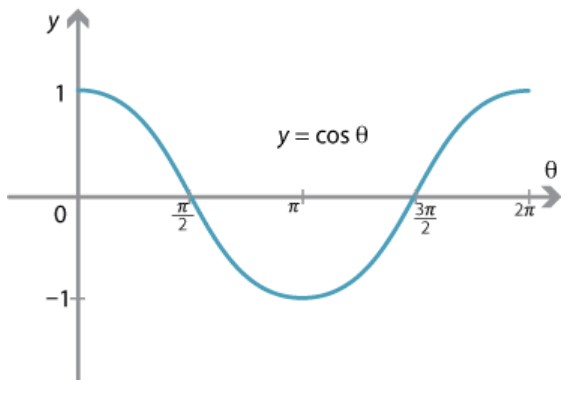
\includegraphics[width = 0.3\textwidth]{media/cosine}
	\end{center}
{\color{defgruen}We also use the notation $\alpha:=\sphericalangle(x,y)$}, since $\alpha$ can be considered´ the angle between $x$ and $y$.	
\end{frame}

\begin{frame}
	
		Geometric insights from the identity 
		$$\text{cosine} = \frac{\text{adjacent}}{\text{hypotenuse}} .$$
\Hide{~\\
		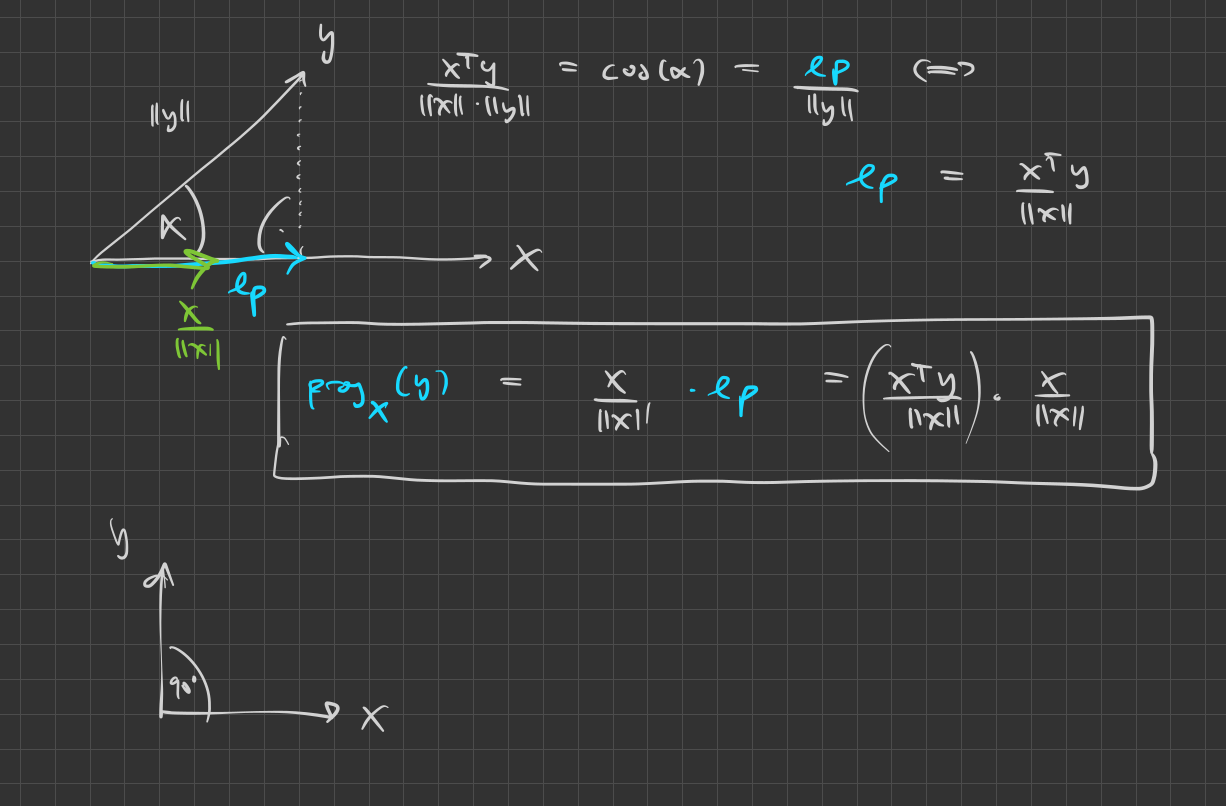
\includegraphics[width=0.95\linewidth]{media/projections}
}
\end{frame}



%%%%%%%%%%%%%%%%%%%%%%%%%%%%%%%%%%%%%%%%%%%%%%%%%%%%%%%%%%%%%%%%%%%%5
% GENERAL NORMS AND INNER PRODUCTS
%%%%%%%%%%%%%%%%%%%%%%%%%%%%%%%%%%%%%%%%%%%%%%%%%%%%%%%%%%%%%%%%%%%%%

%\elomath{
%\begin{frame}
%	\Hide{
%		~\\
%		normalization, unit circle: 3 pictures (simple, rotated, general+projection)\\
%		-- (1) $x$ = unit vector\\ 
%		(2) you can always rotate $x$ to the unit vector (this rotation depends on $x$ and has to be applied to $y$, so that $y_1$ changes to a $\tilde{y}_1(x) = x^Ty$):\\~\\
%		-- relation to projections,
%		$$\frac{x^Ty}{\|x\|_2\cdot\|y\|_2} = \cos(\alpha) = \frac{\ell}{\|y\|_2} ~~\Leftrightarrow~~ \ell = \frac{x^Ty}{\|x\|_2} $$
%		We define: $$\text{proj}_x(y) := \frac{x^Ty}{\|x\|_2} \frac{x}{\|x\|_2} $$ 
%		~\\
%		-- allude to orthogonality
%	}
%\end{frame}
%\begin{frame} 
%\pictures{
%	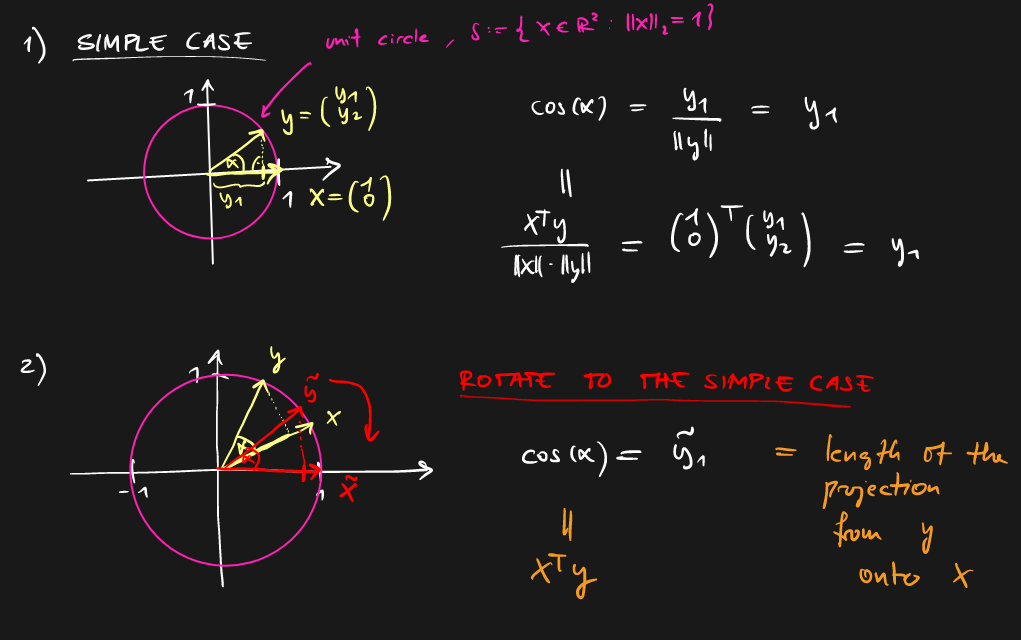
\includegraphics[width=0.7\textwidth]{media/innerproduct-as-projection1}\\
%	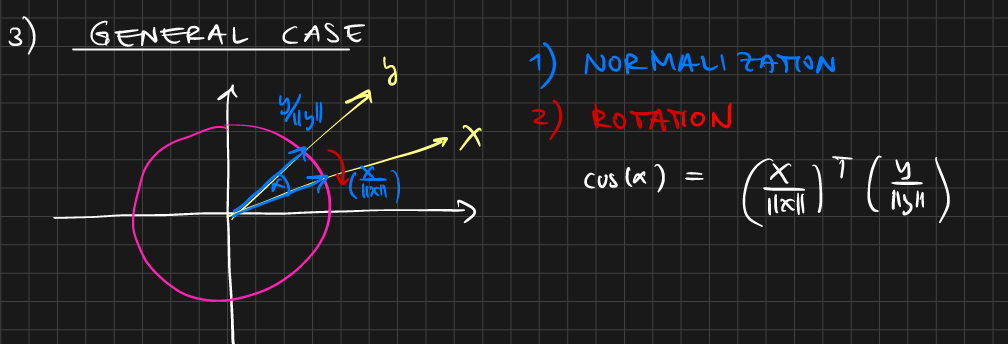
\includegraphics[width=0.7\textwidth]{media/innerproduct-as-projection2}
%}
%\end{frame}
%}



%\only<article>{
%	{\large \textbf{Question:} Do all ($p$-)norms correspond to an inner product?}
%	\begin{lemma}[Polarization identity]\label{lem:polarization}
%		Let $(\cdot,\cdot)\colon \R^n\times \R^n \to \R$ be an inner product on $\R^n$ and $\|\cdot\|\colon \R^n \to [0,\infty)$, $\|v\| := \sqrt{(v,v)}$. Then
%		\[
%		(v,w)=\frac14\left(\|v+w\|^2-\|v-w\|^2\right).
%		\]
%	\end{lemma}
%	%
%	%
%	\begin{re}
%		By Corollary \ref{cor:innerproduct_defines_norm} each inner product induces a norm. However, with the help of Lemma \ref{lem:polarization} one can show that, e.g., the norms $\|\cdot\|_1$ or $\|\cdot\|_\infty$ are not induced by an inner product, i.e., there is no mapping $(\cdot,\cdot)$ satisfying Definition \ref{def:innerproduct} so that $\|v\|_1 = \sqrt{(v,v)}$.
%	\end{re}
%	interpretation in terms of angle
%
%\begin{frame}
%\Subsection{Scalar product and Norm}
%%
%\begin{itemize}
%	\item \textbf{Question:} Can we ``solve'' a linear system, where the matrix is not invertible or even not quadratic? -- in which sense? \\
%	$\rightarrow$ this is the topic of the following two sections.
%	\item \textbf{Recall:}\\
%	$Ax=b$ solvable ~~$\Leftrightarrow$~~ $A\in GL_n(\F )$, which means $x=A^{-1}b$~~ $\Rightarrow$~~ $Ax-b=0$ 
%	\item 
%	\textbf{Idea:} What about making $Ax-b\in\F^n$ just very small, if $A$ is any matrix?
%	\item {\bf What is a small vector?}\\ 
%	We need a length mapping $L:\F^n\to [0,\infty)$ with some plausible properties:
%	\ite
%	\item[(i)] $L(v)=0\ \Rightarrow v=0$ ~~\textit{(positive definite/ point separating)}
%	\item[(ii)] $L(r\cdot v)=|r|\cdot L(v)\, ,\ \forall v\in\F^n, r\in\R$~~\textit{(absolutely homogeneous)}
%	\item[(iii)] $L(v+w)\le L(v)+L(w), \ \forall v,w\in\F^n$ \textit{(subadditive/ triangle inequality)}
%	\eti
%\end{itemize}
%
%\begin{defi}[Norm] \label{def:norm} If a mapping $L\colon\F^n\to[0,\infty)$ satisfies properties (i)-(iii), then it is called a \textbf{norm} and we use the notation
%	$\|v\|:=L(v)$ for $v\in \F^n$. 
%\end{defi}
%\begin{itemize}
%	\item[$\rightarrow$] There are a lot of norms available. For the moment, we focus on the most often used norm and also only on vectors from $\R^n$.
%\end{itemize}
%\Hide{ Example in $\R$: Absolute value $|x|$ for $x\in \R$.}
% 
%\end{frame}
%
%\begin{frame} 
%The standard norm for $x \in \R^n$ is introduced in the following definition.
%\begin{defi}[$p$-norm] \label{def:pnorm}
%	Let $x\in \R^n$ and $p \in [1,\infty]$. Then the $p$-norm $\|\cdot\|_p\colon \R^n \to [0,\infty)$ is defined by
%	\begin{align}
%	\norm{x}_{p} = \left(\sum_{i=1}^n \abs{x_{i}}^p\right)^\frac{1}{p}. \label{def:pnorm}
%	\end{align}	 
%\end{defi}
%\vspace{-0.45cm}
%\begin{ex}
%	\blank
%	\begin{align*}
%	\underline{p=1}: ~~~~&~\norm{x}_{1} = \sum\limits_{i=1}^n \abs{x_{i}} &\text{Manhattan norm}\\
%	\underline{p=2}:~~~~~ &~\norm{x}_{2} = \sqrt{\sum\limits_{i=1}^n x_{i}^2} &\text{Euclidean norm}\\
%	\underline{p=\infty}: ~~~~~&~\norm{x}_{\infty} := \lim\limits_{p \rightarrow \infty} {\norm{x}_{p}} = \max_{i \in \set{1,..,n}}{\abs{x_{i}}} &\text{Maximum norm}
%	\end{align*}
%\end{ex}
%{
%	\blank
%	Proof for identity with $p=\infty$\\
%	w.l.o.g. we assume that $\abs{x_{1}}$ is maximal. There are may b $k$ further entries with $\abs{x_{i}} = \abs{x_{1}}$ then \\
%	$\norm{x}_{p} = \left(\sum\limits_{i=1}^n {\left|x_{i}\right|}^p\right)^\frac{1}{p} = \abs{x_{1}} \left(k + \underbrace{{\left|\frac{x_{k+1}}{x_{1}}\right|}^p}_{\rightarrow 0} + \cdots +\underbrace{{\left|\frac{x_{n}}{x_{1}}\right|}^p}_{\rightarrow 0}\right)^\frac{1}{p} \longrightarrow \abs{x_{1}}$
%	
%	for any $k\in \mathbb{N}$ we have $\sqrt[p]{k} \rightarrow 1, p \rightarrow \infty$ 
%}
%\end{frame}
%
%
%%
%\begin{lemma}
%	The $p$-norm $\|\cdot\|_p$ from \eqref{def:pnorm} is indeed a norm as introduced in Definition \ref{def:norm}.
%\end{lemma}
%\begin{proof}
%	\blank
%	We exemplary proof this statement for $p\in \{1,2,\infty\}$ (for general proof conduct any linear algebra book). For this purpose we need to verify the three requirements that a norm shall satisfy.	\\ 
%	\textbf{For $1$-norm}\\
%	\begin{align*}
%	\text{Assume w.o.l.g.}\; &v_1 \neq 0 \Rightarrow \abs{v_1}>0 \Rightarrow \sum\limits_{i=1}^n \underbrace{\abs{v_i}}_{\ge 0} \geq \abs{v_1} > 0\\
%	0 = \norm{v}_{1} = &\sum\limits_{i=1}^n \underbrace{\abs{v_{i}}}_{\geq 0} \Rightarrow v_{i} = 0, \forall{i} \Rightarrow v=0\\
%	\norm{r\cdot v}_{1} = &\sum\limits_{i=1}^n \abs{r \cdot v_{i}} = \sum\limits_{i=1}^n \abs{r} \cdot \abs{v_{i}} = \abs{r}\sum\limits_{i=1}^n \abs{v_{i}} = \abs{r}\cdot \norm{v}_{1}\\
%	\norm{v+w}_{1} = &\sum\limits_{i=1}^n \abs{v_{i}+w_{i}} \leq \sum\limits_{i=1}^n (\abs{v_{i}} + \abs{w_{i}}) = \sum\limits_{i=1}^n \abs{v_{i}} + \sum\limits_{i=1}^n \abs{w_{i}} = \norm{v}_{1} + \norm{w}_{1}
%	\end{align*}
%	\textbf{For $\infty$-Norm}: analogous arguments as for the 1-norm.\\
%	\textbf{For $2$-norm}\\
%	later
%	\begin{align*}
%	0 = \norm{v}_{2} = &\sqrt{\sum\limits_{i=1}^n v_{i}^2} \Rightarrow 0 = \sum\limits_{i=1}^n v_{i}^2 \Rightarrow v_{i}^2 = 0, \forall{i} \Rightarrow v_{i}=0, \forall{i} \Rightarrow v = 0\\
%	\norm{r\cdot v}_{2} = &\sqrt{\sum\limits_{i=1}^n (r \cdot v_{i})^2} = \sqrt{\sum\limits_{i=1}^n  r^2 \cdot v_{i}^2} = \sqrt{r^2\sum\limits_{i=1}^n \cdot v_{i}^2} = \abs{r}\sqrt{\sum\limits_{i=1}^n v_{i}^2} = \abs{r}\norm{v}_{2}\\
%	\norm{v+w}_{2} &\leq \norm{v}_{2} + \norm{w}_{2}
%	\end{align*}
%	triangle inequality more difficult (later)\\~\\
%\end{proof}
% 
%\begin{frame} 
%%
%\begin{defi}[Inner product]\label{def:innerproduct}
%	A mapping $(\cdot,\cdot)\colon \R^n\times \R^n \to \R$ is called \textbf{inner product} (or \textbf{scalar product}) on $\R^n$ if it satisfies
%	\begin{itemize}
%		\item[(i)] $\forall v,w \in \R^n: ~(v,w) = (w,v)$~~~~~~~~~~~~~~~~~~~~~~~~~~~~~~~~~~~~~~~~~~(symmetric)
%		\item[(ii)]$\forall v,w_1,w_2 \in \R^n: ~(v,w_1+w_2) = (v,w_1)+(v,w_2)$
%		\item[] $\forall v,w \in \R^n, r \in \R: ~ (v,r\cdot w)=r\cdot(v,w)$~~~~~~~~~~~~~~~~~~~~~~~~~~~~~~(linear in its second argument)
%		\item[(iii)] $\forall v \in \R^n\backslash\{0\}: ~ (v,v) > 0$ ~~~~~~~~~~~~~~~~~~~~~~~~~~~~~~~~~~~~~~~~~~~~~(positive definite)
%	\end{itemize}
%	%
%\end{defi}
%~\\
%{\large \textbf{Question:} Relation between norms and inner products?}
%\begin{theo}[Cauchy-Schwarz inequality]\label{theo:cauchyschwarz}
%	Let $(\cdot,\cdot)\colon \R^n\times \R^n \to \R$ be an inner product on $\R^n$ and $\|\cdot\|\colon \R^n \to [0,\infty)$, $\|v\| := \sqrt{(v,v)}$. Then there holds the \textbf{Cauchy-Schwarz inequality}: 
%	$$\left|(v,w)\right|\le \|v\|\cdot\|w\|.$$
%\end{theo}
%\begin{proof}
%	\blank
%	Property (3) is shown via Cauchy-Schwarz inequality, which is trivially correct, if $v=0$ or $w=0$. Now, we assume that both are nonzero. Obviously, $z^\top z\ge 0$, for any $z\in\R^n$. We choose $z:=v/\|v\|_2-w/\|w\|_2$ and achieve
%	\[
%	0\le z^\top z=\frac{v^\top v}{\|v\|_2^2}-2\frac{v^\top w}{\|v\|_2\cdot\|w\|_2}+\frac{w^\top w}{\|w\|_2^2}=2-2\frac{v^\top w}{\|v\|_2\cdot\|w\|_2}
%	\Rightarrow \left|v^\top w\right|\le \|v\|_2\cdot\|w\|_2
%	\]
%\end{proof}
%\end{frame}
%
%
%\begin{frame} 
%\textbf{We find:} Each inner product defines a norm.
%\begin{corollary} \label{cor:innerproduct_defines_norm}
%	Let $(\cdot,\cdot)\colon \R^n\times \R^n \to \R$ be an inner product on $\R^n$, then $\|\cdot\|\colon \R^n \to \R$,
%	$$\|v\| := \sqrt{(v,v)}$$ 
%	defines a norm on $\R^n$.
%\end{corollary}
%\begin{proof}
%	\blank
%	Properties (1) and (2) are obvious. 
%	C-S leads to $\|v+w\|_2^2=(v+w)^\top(v+w) = v^Tv +  2v^Tw+w^Tw\le v^Tv +  2\norm{v}_2\norm{w}_2+ w^Tw\le(\|v\|_2+\|w\|_2)^2$, which is the triangle inequality.
%\end{proof}
%%
%\end{frame}
%%
%}
%
%
%
%
%\only<article>{
%\begin{frame} 
%{\large \textbf{Question:} Can we characterize \emph{all} inner products on $\R^n$?}
%\begin{defi}[Symmetric and positive definite matrices]
%	Let $A \in \R^{n\times n}$. 
%	\begin{itemize}
%		\item[(i)] $A$ is called \textbf{symmetric}, if $A = A^T$.
%		\item[(ii)] $A$ is called \textbf{positive definite}, if $v^\top Av>0\, ,\ \forall v\in\R^n\setminus\{0\}$.
%	\end{itemize}
%	We define the set of all symmetric and positive definite matrices by $$\R^{n\times n}_{spd} := \{ A \in \R^{n\times n}\colon A~ \text{sym and pos. def.}\}\subset GL_n(\R) \subset \R^{n\times n}.$$
%\end{defi}
%\begin{theo}[Characterization]\label{theo:characterization_inner_products}
%	Let $(\cdot,\cdot)\colon \R^n\times \R^n \to \R$ be a mapping on $\R^n$. Then:
%	$$ (\cdot,\cdot) ~~\text{inner product}~~ \Leftrightarrow ~~\exists A \in \R^{n\times n}_{spd}\colon (v,w) = (v,w)_A := v^TAw ~~\forall v,w\in \R^n. $$
%	%A symmetric and positive definite matrix $A\in\R^{n\times n}$ defines a scalar product $(v,w)_A:=v^\top Aw$. On the other hand, any scalar product $(v,w)$ can be written as $(v,w)=v^\top Aw$ with an appropriate symmetric and positive definite matrix $A$.
%\end{theo}
%\end{frame}
%
%\begin{frame}
%\begin{proof} 
%	\blank	
%	``$\Leftarrow$'' obvious. ``$\Rightarrow$'' is shown by the construction:
%	\[
%	A=[a_{ij}]_{ij}\, , \qquad a_{ij}:=(e_i,e_j)\text{, where } e_i:=
%	\bbmat \delta_{1,i}, \ldots , \delta_{n,i}\ebmat^\top
%	\]
%	\begin{itemize}
%		\item[a)] let A be symmetric and positive definite: i.e. $A^T = A$ and $v^T Av > 0, \forall{v \neq 0}$
%		\begin{enumerate}
%			\item[(i)] $(v,w)_A = v^T Aw = (v^T Aw)^T = w^T A^T v = w^T Av = (w,v)_A$
%			\item[(ii),(iii)] $(v, \alpha w_1 + \beta w_2)_A = v^T A(\alpha w_1 + \beta w_2) = v^T A(\alpha w_1) + v^T A(\beta w_2) = \alpha v^T Aw_1 + \beta v^T Aw_2 = \alpha(v,w_1)_A + \beta(v,w_2)_A$
%			\item[(iv)] $(v,v)_A^{\frac{1}{2}} = (v^T Av)^{\frac{1}{2}}$
%		\end{enumerate}
%		\begin{align*}
%		\text{norm(1):}\;\; &0 = (v,v)_A^{\frac{1}{2}} = (v^T Av)^{\frac{1}{2}} \Rightarrow v=0,\; \text{because A is p. d.}\\
%		\text{norm(2):}\;\; &(r\cdot v, r\cdot v)_A^{\frac{1}{2}} = [(r\cdot v)^T A(r\cdot v)]^{\frac{1}{2}} = [r^2 v^T Av]^{\frac{1}{2}} = \mid r \mid (v,v)_A^{\frac{1}{2}}\\
%		\text{norm(3):}\;\; &\text{triangle inequality: can be shown for}\; (.,.)_A^{\frac{1}{2}}\; \text{as for} \;\norm{}_2\; \\&\text{by generalizing Cauchy-Schwartz (T.4.4) to} (.,.)_A\\
%		\end{align*}
%		\item[b)] any $v \in \mathbb{R^n}$ is given as $v  = \sum\limits_{i=1}^n v_i e_i$ , similar: $w = \sum\limits_{i=1}^n w_i e_i$\\[5pt]
%		$\begin{pmatrix}
%		        v_{1} \\
%		        v_{2} \\
%		        \vdots \\
%		        v_n 
%		    \end{pmatrix} = v_1 \begin{pmatrix}
%		        1 \\
%		        0 \\
%		        0 \\
%		        \vdots \\
%		        0 
%		    \end{pmatrix} + v_2  \begin{pmatrix}
%		        0 \\
%		        1 \\
%		        0 \\
%		        \vdots \\
%		        0 
%		    \end{pmatrix} + \cdots + v_n  \begin{pmatrix}
%		        0 \\
%		        0 \\
%		        0 \\
%		        \vdots \\
%		        1 
%		    \end{pmatrix}  $
%		$\Rightarrow (v,w) = (\sum\limits_{i=1}^n v_i e_i, \sum\limits_{j=1}^n w_j e_j)$\\[5pt]
%		$=\sum\limits_{i=1}^n v_i \sum\limits_{j=1}^n w_j (e_i,e_j)$\\[5pt]
%		$=\sum\limits_{i=1}^n \sum\limits_{j=1}^n v_i\underbrace{(e_i, e_j)}_{A:=[(e_i,e_j)]_{ij}} w_j = v^T Aw$\\[5pt]
%		This matrix is obviously s. p. d.
%	\end{itemize}
%\end{proof}
%\end{frame}
%}


% ORTHOGONAL MATRIX
\begin{frame}
\Subsection{Orthogonal Vectors and Matrices}
Let us again consider the relation 
$$\cos(\alpha) = \frac{x^Ty}{\|x\|_2\cdot\|y\|_2},~~~x,y\in\Rn  .$$
Now let us assume that the angle $\alpha = \sphericalangle(x,y)$ between the two vectors $x,y$ is $90^\circ$, i.e., $\alpha =\pm \frac{\pi}{2}$, meaning that they are \textit{perpendicular}. Then we find
\begin{equation*}
 ~~~0 = \cos\left(\pm \frac{\pi}{2}\right) = \frac{x^Ty}{\|x\|_2\cdot\|y\|_2}  
 ~~~~~~\Leftrightarrow~~~~~~ 0 = x^\top y.
\end{equation*}
~\\~\\
In mathematics we call this \textit{orthogonal} and make it a general definition:\vspace{-0.25cm}
\begin{defi}[Orthogonal/-normal vectors]~\\
\begin{itemize}
	\item[i)] Two vectors $x,y \in \F^n$ are called \textbf{orthogonal} if $(x,y)_2 = x^H y  = 0$.
	\item[ii)] Two vectors $x,y \in \F^n$ are called \textbf{orthonormal} if they are orthogonal and have length $1$ (i.e., $\|x\|_2=\|y\|_2=1$).
	\item[iii)] Vectors $x_1, \ldots, x_r \in \F^n$ are called (mutually) \textbf{orthogonal (orthonormal)} if $x_i, x_j$ are \textbf{orthogonal (orthonormal)} for all possible pairs $i\neq j \in \{ 1,\ldots, r\}$.
\end{itemize} 
\end{defi} 
~\\
{\color{satzrot} One can show that:
\begin{equation}\label{eq:orthoImpliesIndepen}
x,y ~~\text{orthogonal} ~~~\Rightarrow ~~~ x,y~~\text{linearly independent} .
\end{equation}
}
\Hide{~\\
%\textbf{Example: Identity matrix; rotate the unit vectors; rotation matrix; reflection?}\\
\small Counter example for backwards implication: $x=\begin{pmatrix}1\\0\end{pmatrix},y=\begin{pmatrix}1\\1\end{pmatrix}$}
\end{frame}

\begin{frame}
	\Hide{
\begin{example} \label{ex:orthogonalVecs}
	~\\
	For $\F=\R$ and $n=2$ consider, e.g.,
	 \begin{itemize}
	 	\item Standard basis vectors.
	 	\item Rotation of the standard basis vectors.
	 \end{itemize}
\end{example}	

}
\end{frame}

\begin{frame}
\textbf{Now let us extend this notion to matrices:}~\\~\\
For this purpose observe that the matrix-matrix product $Q^HQ$ for $Q \in \F^{n \times n}$ contains all possible inner products of its columns:\\
\Hide{
	~\\
{\centering
$
\underbrace{\begin{pmatrix}
	-&\overline{q_1}^\top&-\\
	-&\overline{q_2}^\top&-\\
	&\vdots& \\
	-&\overline{q_n}^\top&-
	\end{pmatrix}}_{Q^H}
\underbrace{\begin{pmatrix}
	|&|& &|\\
	q_1&q_2&\cdots&q_n\\
	|&|& &|
	\end{pmatrix}}_{Q}
=\begin{pmatrix}
q_1^Hq_1&\cdots&q_1^Hq_n\\
q_2^Hq_1&\cdots&q_2^Hq_n\\
\vdots&\ddots&\vdots\\
q_n^Hq_1&\cdots&q_n^Hq_n
\end{pmatrix}
~~~~~\left(=\begin{pmatrix}
1&0&\cdots&0\\
0&1&\ddots&\vdots\\
\vdots&\ddots&\ddots&0\\
0&\cdots&0&1
\end{pmatrix}\right)
$
~\\
}
}
%~\\\vspace{3cm}
~\\Let us assume that the columns of $Q$ are mutually ortho\textit{normal}, then $$Q^HQ = I_n .$$
Since this is a central property, we make this a definition:\vspace{-0.25cm}
\begin{defi}[Orthogonal/Unitary matrix]
	A matrix $Q\in\F^{n\times n}$ is called \textbf{\emph{unitary}}, if $$Q^HQ =I_n.$$\\
	For a real matrix $Q\in\R^{n\times n}$ this condition simplifies to $Q^TQ =I_n$, in which case we then call the matrix \textbf{\emph{orthogonal}}.
\end{defi}
\Hide{
Since orthogonality implies linear independence (see statement \eqref{eq:orthoImpliesIndepen}) we know that \textbf{orthogonal matrices are invertible}. From the defining equation $Q^T Q=I_n$ we can even deduce its inverse
 $$  Q^{-1} = Q^T$$ and therefore also $QQ^T=I_n$.\\
 \vspace*{0.2cm}
 $\rightarrow$ This is one (of the many) reasons why the property of orthogonality is very desirable.
}
\end{frame}


\begin{frame}
	\textbf{Understanding $QQ^\top(\cdot)$ as orthogonal projection}~\\~\\
	\Hide{
	For a vector $q \in \Rn$ of length $1$, i.e., $\|q\|_2=1$, and a vector $y\in\Rn$ we find
	$$\text{proj}_q(y) =  (q^\top y) \cdot q.$$
	Now let $Q = [q_1,\ldots, q_n]\in\Rnn$ be an orthogonal matrix (i.e., columns $q_i$ are mutually orthonormal), then
	$$y = I \cdot y 
	=  QQ^\top y 
	= Q \begin{pmatrix}
	q_1^\top y \\ \vdots \\ q_n^\top y
	\end{pmatrix}
	= \sum_{i=1}^n q_i^\top y \cdot q_i
	= \sum_{i=1}^n \text{proj}_{q_i}(y).$$
	With other words, in order to obtain the coordinates of $y$ with respect to the \textit{orthonormal} basis $\{q_1,\ldots, q_n\}$ we solely have to project $y$ onto each basis vector $q_i$.
	\Vspace{1cm}
	\textbf{Example}\\
	Famous related examples from signal processing include the Discrete Cosine Transform (DCT) and the Discrete Fourier Transform (DFT) which can be written as a matrix--vector product $Q^\top(\cdot)$ with an orthogonal/unitary matrix $Q$. In this context, the $q_i$ may correspond to discrete periodic functions of different frequency. For a time-discrete signal 
	$$y=(y_1,\ldots, y_n)^\top \in \Rn$$ 
	one says that the transformed signal 
	$$Q^\top y = (q_1^\top y,\ldots,q_n^\top y)^\top$$ 
	lives in the frequency space.
	
%TODO
%keep?
%	\textbf{Characterization of orthogonal matrices:}\\[0.2cm]
%\textit{Orthogonal matrices are matrices which do not change angle or length, i.e., }
% \begin{itemize}
% 	\item \textit{isometric}: $\|Qx\|_2 = \|x\|_2$
% 	\item \textit{isogonic}: $(Qx, Qy)_2 = (x,y)_2$
% \end{itemize}
%\vspace{0.3cm}
%More precisely, \textit{Reflections} and \textit{rotations} (and combinations).
}
\end{frame}

\begin{frame}[c]
	\centering
	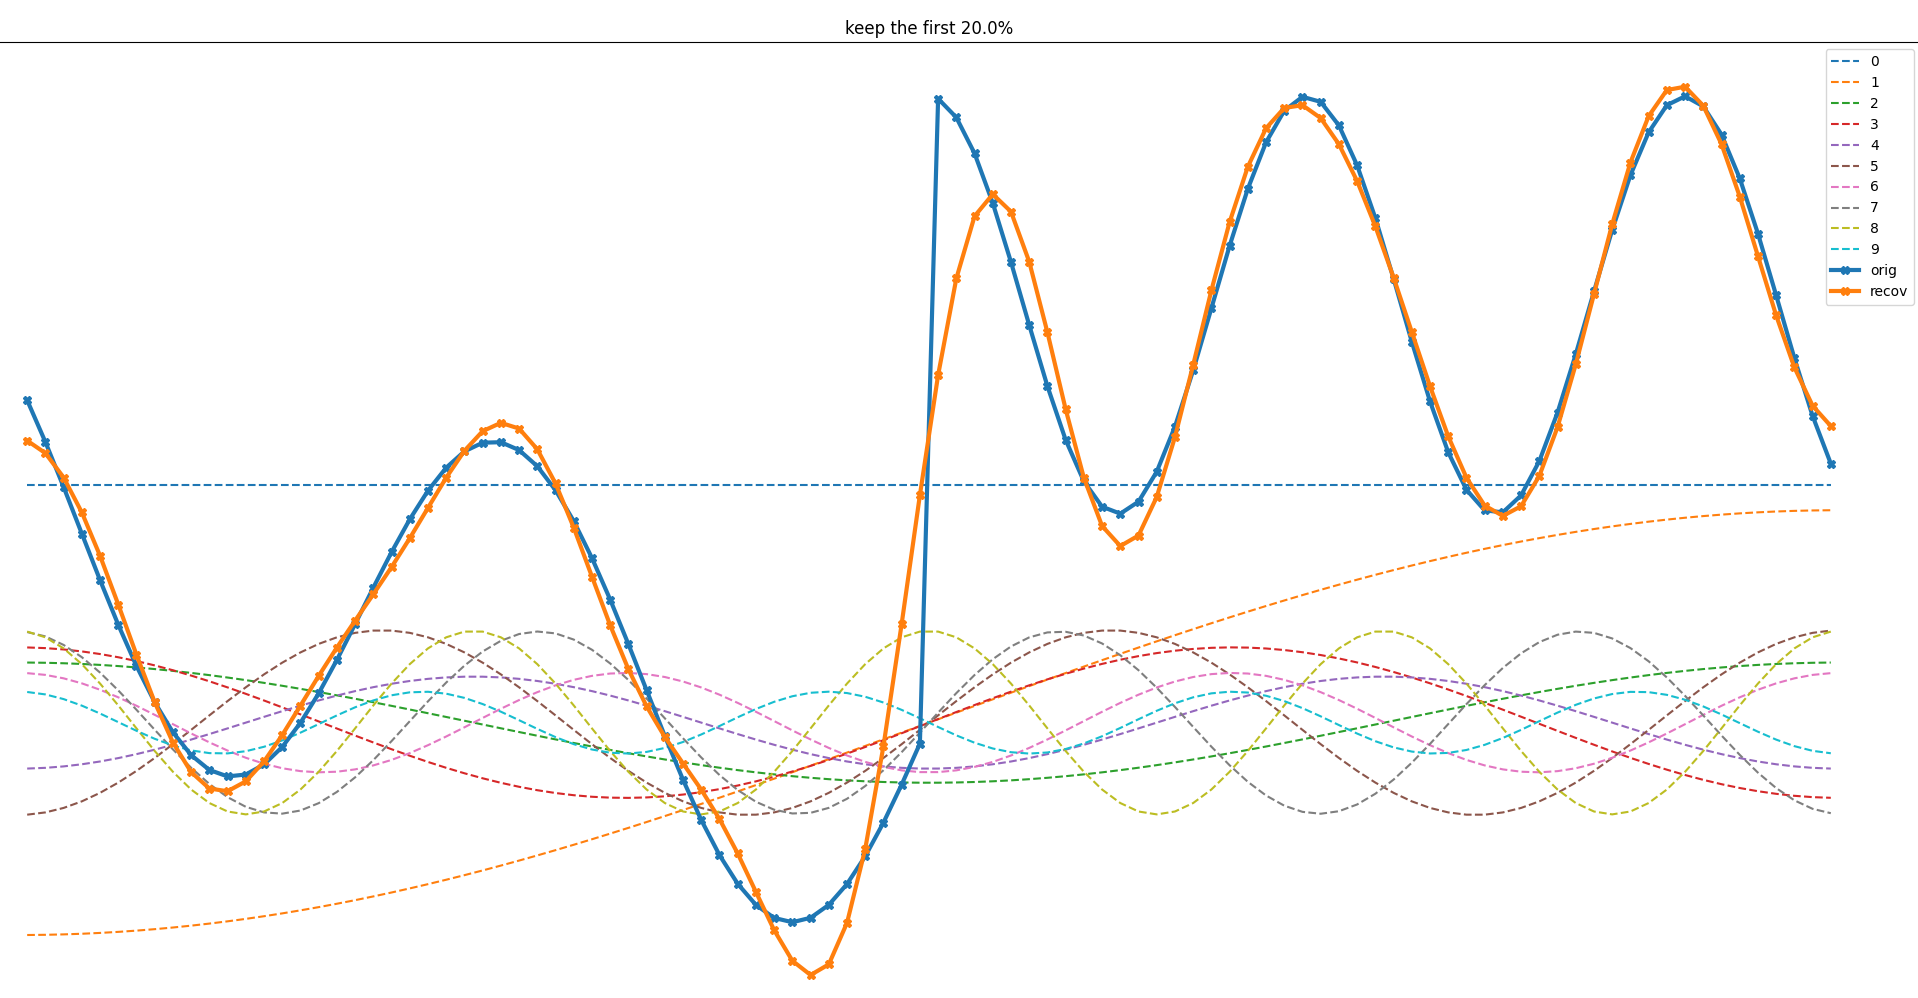
\includegraphics[width=0.99\textwidth]{./media/dct-1d.png}
	1-d DCT compression example (where high frequencies are removed):
	$$
	y 
	= \sum_{i=1}^n q_i^\top y \cdot q_i
	\approx \sum_{i=1}^m q_i^\top y \cdot q_i ~~~(m<n).$$
\end{frame}
\begin{frame}[c]
	\centering
	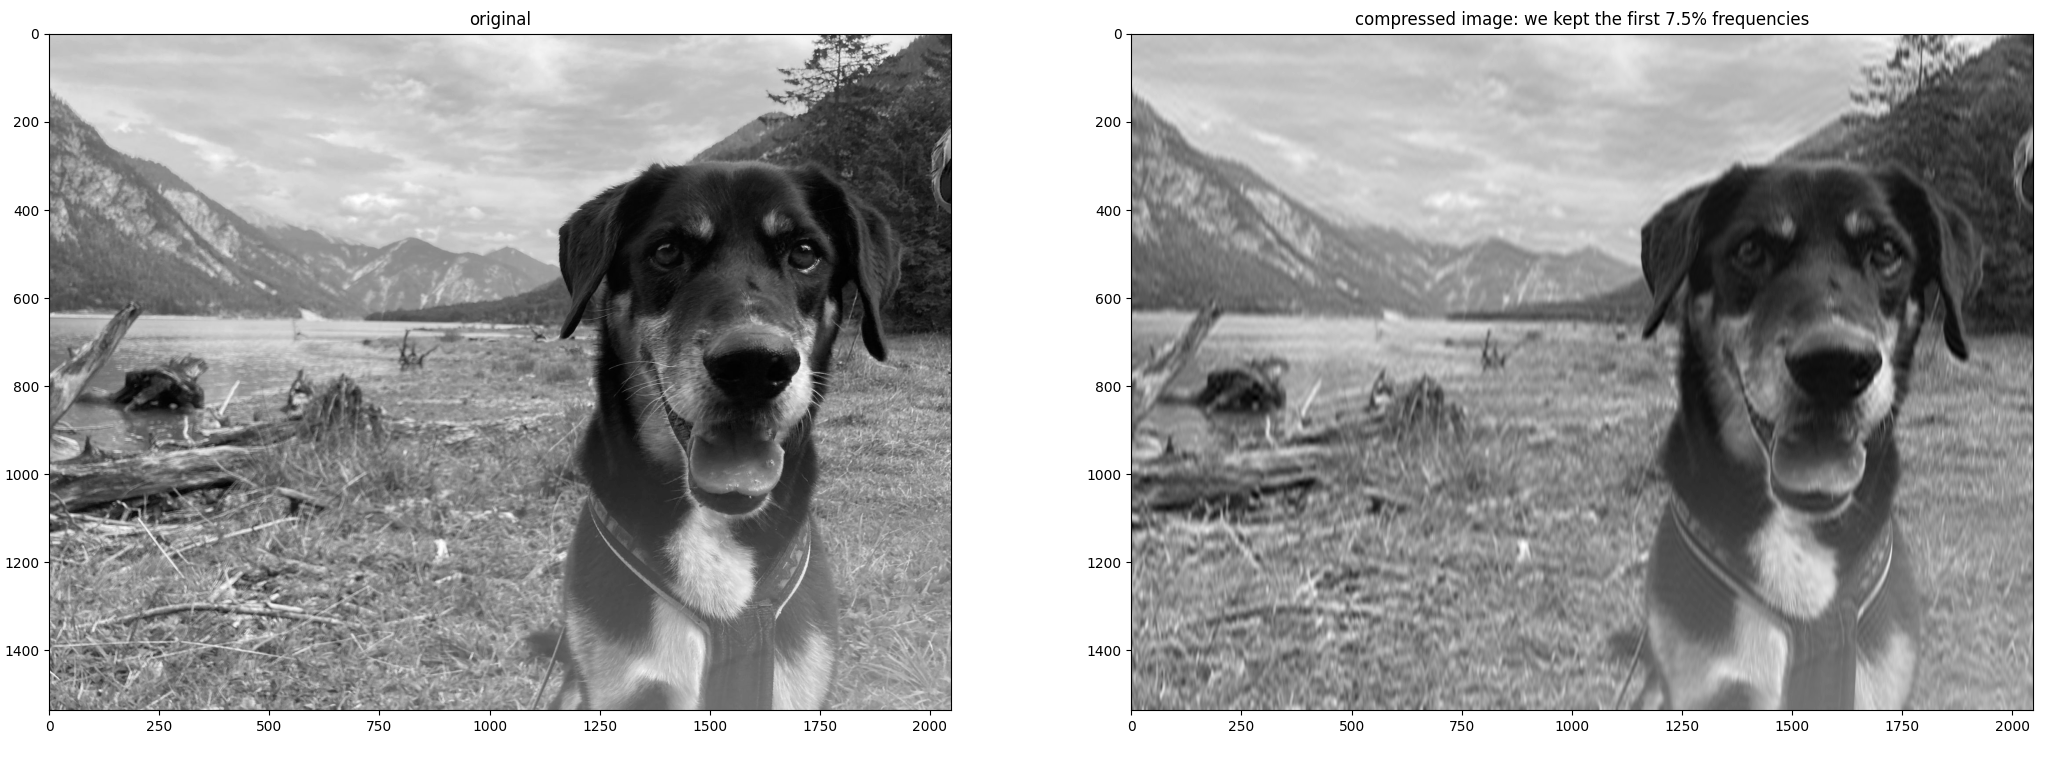
\includegraphics[width=0.99\textwidth]{./media/dct-2d.png}
	2-d DCT compression example (where high frequencies are removed)
\end{frame}


 \begin{frame}
 \Subsection{The Determinant}
  \textbf{Aim:} 
  For $n$ vectors in $\F^n$ we want to have a \textit{measure of linear independence}\\[0.1cm]
  -- or equivalently a \textit{volume measure} for the parallelotope spanned by these vectors  ~\\[0.1cm]
  -- or equivalently a \textit{measure for the invertibility} of a matrix in $\F^{n\times n}$~\\
  	\Hide{~\\
  		\small	Why are all these measures the same?\\
  		\begin{itemize}
  			\item $n$ linear dependent vectors do not span a volume in $\Fn$.
  			\item Linear independent columns of a quadratic matrix imply invertibility.
  		\end{itemize}
  	\pictures{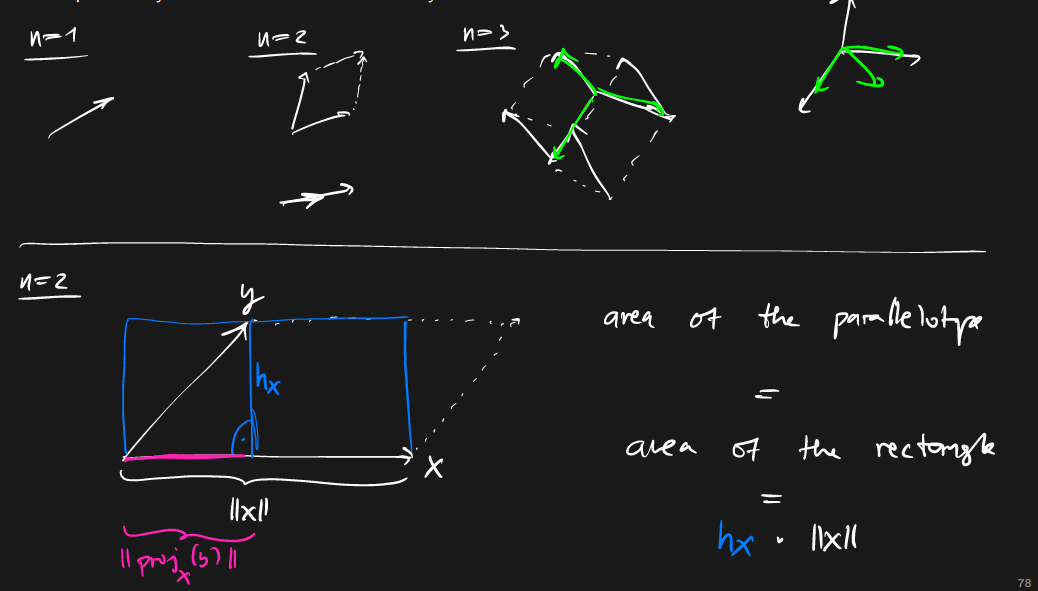
\includegraphics[width=0.8\textwidth]{media/determinant}}}
\end{frame}

%%
\begin{frame}
	\Hide{\small
Let us derive a formula in the two--dimensional case: Let 
	\begin{center}
		$a := $ area of the parallelogram $=$ area of rectangle $= h_x \cdot \|x\|_2$.
	\end{center}
	By the Pythagorean identity we obtain: 
	\begin{align*}
	h_x^2 + \|\text{proj}_x(y)\|_2^2 &= \|y\|_2^2\\
	\Leftrightarrow h_x^2 & =\|y\|_2^2 - \|\text{proj}_x(y)\|_2^2
	=\|y\|_2^2 - \frac{(x^Ty)^2}{\|x\|_2^2}\\
	&= \frac{\|y\|_2^2\|x\|_2^2 - (x^Ty)^2}{\|x\|_2^2} \\
	&= \frac{(y_1^2 + y_2^2)(x_1^2+x_2^2) - (x_1y_1 + x_2y_2)^2}{\|x\|_2^2}\\
	& = \ldots \\
	&=   \frac{(x_1y_2 -x_2y_1)^2}{\|x\|_2^2}.
	\end{align*}
	Thus $$h_x = \left|\frac{x_1y_2 -x_2y_1}{\|x\|_2} \right| = \frac{\left|x_1y_2 -x_2y_1\right|}{\|x\|_2} , $$ which implies $$a = |x_1y_2 -x_2y_1| =: |\det(A)|.$$
}
\end{frame}

% FORMULA FOR THE DETERMINANT
\begin{frame}
In general, there is the following (recursive) formula, which we use as the definition here: \vspace{-0.2cm}
\begin{definition}[Laplace formula]\label{def:Laplace-formula} Let
$A \in \F^{n\times n} $ 
and let
$ A_{ij} \in \F^{(n-1) \times (n-1)} $ be
the matrix resulting from erasing the $i$-th row and $j$-th column. Then the mapping $\det\colon \F^{n\times n} \to \F $ defined by
%
\[
\det(A) = \sum^n_{j=1}(-1)^{i + j} a_{ij} \det(A_{ij})\, ,\quad \text{for a fixed but arbitrary} ~~i \in \left\{1, \ldots, n \right\},
\]
is called the \textbf{determinant} (of $A$), where $\det(a) := a$ for $a\in\R = \R^{1\times 1}$.
\end{definition}
{\color{satzrot} One can show: The determinant is a well-defined function, i.e., by the formula above the function $\det(\cdot)$ assigns to each matrix $A \in \Fnn$ exactly one number in $\F$.}\\
\vspace{0.5cm}
\textbf{Laplace formula for $n=2$ and $n=3$:}\\\vspace{0.2cm}
$\bullet~ n=2$ ~{\small (we fix $i=1$)}  \\ \vspace{0.2cm}
\Hide{Here we have $$ \det(A) =\sum^2_{j=1}(-1)^{1 + j} 
a_{1j} \det (A_{1j})$$ 
{\footnotesize $A_{11} = \begin{pmatrix}
	\textcolor{red}{a_{11}} & \textcolor{red}{a_{12}}\\
	\textcolor{red}{a_{21}} & a_{22}
	\end{pmatrix} = [a_{22}],~~
	A_{12} = \begin{pmatrix}
	\textcolor{red}{a_{11}} & \textcolor{red}{a_{12}}\\
	a_{21} & \textcolor{red}{a_{22}}
	\end{pmatrix} = [a_{21}] $,~~
    $A_{21} = \begin{pmatrix}
	\textcolor{red}{a_{11}} & a_{12}\\
	\textcolor{red}{a_{21}} & \textcolor{red}{a_{22}}
	\end{pmatrix} = [a_{12}], ~~
	A_{22} = \begin{pmatrix}
	a_{11} & \textcolor{red}{a_{12}}\\
	\textcolor{red}{a_{21}} & \textcolor{red}{a_{22}}
	\end{pmatrix} = [a_{11}] $}\\[0.5cm]
So that all in all
$$ \det(A) = (-1)^{1+1} a_{11} \det(A_{11}) + (-1)^{1+2} a_{12} \det(A_{12}) = a_{11} \cdot a_{22} - a_{12}\cdot a_{21}$$ 
% \underline{2nd option:} $\det(A) = (-1)^{2+1} a_{21} \det(A_{21}) + (-1)^{2+2} a_{22} \det(A_{22}) = -a_{21}\cdot a_{12} + a_{22}\cdot a_{11}$
}
~\\
$\bullet~ n=3:$ \textit{Sarrus rule} (exercise)
\only<article>{
	\begin{itemize}
		\item[] $\det(A)=\det\left(\begin{pmatrix}
		\textcolor{cyan}{a_{11}} & \textcolor{orange}{a_{12}} & \textcolor{cyan}{a_{13}}\\
		\textcolor{orange}{a_{21}} & \textcolor{cyan}{a_{22}} & \textcolor{orange}{a_{23}}\\
		\textcolor{cyan}{a_{31}} & \textcolor{orange}{a_{32}} & \textcolor{cyan}{a_{33}}
		\end{pmatrix}\right)$\\
		\item[] $ = a_{11} \cdot det\begin{pmatrix}
		\textcolor{cyan}{a_{22}} & \textcolor{orange}{a_{23}} \\
		\textcolor{orange}{a_{32}} & \textcolor{cyan}{a_{33}}
		\end{pmatrix} - a_{12} \cdot det\begin{pmatrix}
		\textcolor{cyan}{a_{21}} & \textcolor{orange}{a_{23}} \\
		\textcolor{orange}{a_{31}} & \textcolor{cyan}{a_{33}}
		\end{pmatrix} + a_{13} \cdot det\begin{pmatrix}
		\textcolor{cyan}{a_{21}} & \textcolor{orange}{a_{22}} \\
		\textcolor{orange}{a_{31}} & \textcolor{cyan}{a_{32}}
		\end{pmatrix}$\\
		\item[] $ = a_{11}(a_{22}a_{33}-a_{23}a_{32})-a_{12}(a_{21}a_{33}-a_{31}a_{23})+  a_{12}(a_{21}a_{32}-a_{31}a_{22}) =$\\
		\item[] $ = a_{11}a_{22}a_{33}-a_{11}a_{23}a_{32}-a_{12}a_{21}a_{33}+ a_{12}a_{31}a_{23}+a_{13}a_{21}a_{32}-a_{13}a_{31}a_{22}$\\
\end{itemize}}
\end{frame}

\begin{frame}
	\vspace{0.2cm}
	\vspace{0.99cm}
	One can show:\vspace{-0.2cm}
	\begin{theorem}[Determinant properties]\label{theo:det-rules} The determinant satisfies the following computational rules:
		\begin{itemize}		
		\vspace{0.2cm}\item[i)] $\forall  A \in \F^{n \times n}:~~~\det(A)\neq 0\, \Leftrightarrow A\in GL(n,\F ) ~(\Leftrightarrow \text{columns of $A$ are linearly independent})$
		\vspace{0.2cm}\item[ii)] $\forall  A \in \F^{n \times n}:~~~\det(A^\top)=\det(A)$
		\vspace{0.2cm}\item[iii)] if 
		$ A \in \F^{m \times m}, 
		B \in \F^{m \times n}, 
		C \in \F^{n \times n}$ 
		and
		
		\begin{equation*}
		M : \; = 
		\left(
		\begin {array} {c c} 
		A & B \\ 
		0 & C 
		\end {array} 
		\right)
		\in \F^{(m + n) \times (m + n)}
		\end{equation*}
		
		then
		$ \det M = 
		\det A \cdot \det C $
		
		\vspace{0.2cm}\item[iv)] $\forall A,A' \in \F^{n \times n}:~~~\det(A\cdot A')=\det(A)\cdot\det(A')$
	\end{itemize}
	\end{theorem}
	~\\~\\
	\Hide{	The central result for us is i).}
\end{frame}

%
\begin{frame}
	\textbf{Question:} Are there matrices for which the computation of the determinant is easy?\\~\\
 Yes, as in many other situations it turns out that orthogonal and triangular matrices are easy to treat! More precisely, we find:
 ~\\
 \begin{corollary}[Triangular matrices]\label{cor:det-triangular}
 	Let $U \in \F^{n\times n}$ be upper triangular, i.e., 
 	$$ U = \begin{pmatrix}
 	u_{11} & x & \cdots & x \\
 	0& u_{22} & & \vdots \\
 	\vdots & & \ddots & x\\
 	0 & \cdots &0 & u_{nn}
 	\end{pmatrix}.$$ Then	
 	$$\det(U) = u_{11} \cdot u_{22} \cdot \hdots \cdot u_{nn}.$$
 		In particular, we find
 	$$
 	U~\text{is invertible}~~\Leftrightarrow~~\text{det}(U)\neq 0~~\Leftrightarrow~~\forall i:~u_{ii}\neq 0
 	$$
 \end{corollary}
 \begin{proof} Exercise:
 	For the product formula apply Theorem \ref{theo:det-rules} iii) inductively. The second part then easily follows from Theorem \ref{theo:det-rules} i).
 \end{proof}



~\\
 \begin{corollary}[Orthogonal matrices]
 	Let $Q \in \R^{n\times n}$ be an orthogonal matrix, then $|\det(Q)| = 1$.
 \end{corollary}
 \begin{proof}
 	From Cor. \ref{cor:det-triangular} we find $\det(I)=1$. Then result follows from Theorem \ref{theo:det-rules} ii) and iv).
 \end{proof} 
\end{frame}

%\mode<article>{
%\begin{frame}
%
%{\bf Motivation:} Measure of independence? We seek a volume measure for parallelotopes of the form ~\\
%$ \R^2 $ 
%\begin{minipage}{0.4\textwidth}
%	\unitlength1cm 
%	\begin{picture}(6,4) 
%	\put(1,0.2){\includegraphics[scale=0.75]{LocalFolder/LocalMedia/9_det1.eps}} 
%	\end{picture} 
%\end{minipage}
%$ \R^3 $ 
%\begin{minipage}{0.4\textwidth}
%	\unitlength1cm 
%	\begin{picture}(6,4) 
%	\put(-0,-0){\includegraphics[scale=0.75]{LocalFolder/LocalMedia/9_det2.eps}} 
%	\end{picture} 
%\end{minipage}
%~\\
%Thus, this volume measure should satisfy the following properties:
%\begin{itemize} \footnotesize
%	\item[\textbf{(D1)}]
%	The {\bf unit cube} with edge length 1 should have volume {\bf{1}},
%	
%	\[ \det 
%	\left( \left[ 
%	e_1, \ldots, e_n 
%	\right] \right) 
%	= \det (I_n) = 1
%	\]
%	
%	\textit{$\rightarrow~$``$ \det$ is normed''}
%	%
%	%
%	\item[\textbf{(D2)}] 
%	If two edges coincide, then the parallelotope is {\bf flat} and  und has {\bf volume 0}, 
%	
%	$$ \det \left( \left[ v_1, \ldots, v_n \right] \right) = 0, \text{~~if there exist~} i \not = j\text{~~with~~}v_i = v_j$$
%	
%	\textit{$\rightarrow~$``$ \det $ is alternating''}
%	%
%	%
%	\item[\textbf{(D3)}] 
%	The volume is {\bf linear} in {\bf each edge direction}, i.e., 
%	$ \det $ is linear in each column,
%	\begin{align*}
%	\det([ 
%	v_1, \ldots, v_i  
%	& + \lambda \; 
%	v_i', v_{i+1}, \ldots, v_n 
%	] ) \\
%	&=  \det \left( \left[ 
%	v_1 , \ldots, v_i ,\ldots, v_n 
%	\right] \right) 
%	+ \lambda \; \det 
%	\left( \left[
%	v_1, \ldots, v_i^\prime,
%	\ldots, v_n 
%	\right] \right) 
%	\end{align*}
%	
%	\textit{$\rightarrow~$``$ \det $ is a multi linear form''}
%\end{itemize}
%\end{frame}
%
%% DEFINITION AND PROPERTIES
%\begin{frame}
%%Skriptseite 3
%\begin{definition}[Determinant]\label{Definition 10.1}
%Let  $ \F $ be a field and $ n \in  \N $. Then, we call a mapping
%$$
%\triangle:  \F^{n \times n} \rightarrow  \F ,~~~
%A \mapsto \triangle (A)
%$$
%the {\bf determinant}, if it satisfies properties  (D1, D2, D3).
%Thus, the determinant is a normed alternating multilinear form.
%
%\bend{definition}
%\begin{theorem}[Determinant rules]\label{det-rules} The determinant is well-defined and uniquely defined by the properties (D1, D2, D3). Furthermore, it satisfies the following computational rules:
%\ite
%\item[(i)] $\forall  A \in \F^{m \times m}:~~~\det(A)\neq 0\, \Leftrightarrow A\in GL(n,\F ) ~(\Leftrightarrow \text{columns of $A$ are linearly independent})$
%\item[(ii)] $\forall  A \in \F^{m \times m}:~~~\det(A^\top)=\det(A)$
%\item[(iii)] if 
%$ A \in \F^{m \times m}, 
%B \in \F^{m \times n}, 
%C \in \F^{n \times n}$ 
%and
%
%\begin{equation*}
%M : \; = 
%\left[ 
%\begin {array} {c c} 
%A & B \\ 
%0 & C 
%\end {array} 
%\right] 
%\in \F^{(m + n) \times (m + n)}
%\end{equation*}
%
%then
%$ \det M = 
%\det A \cdot \det C $
%
%\item[(iv)] $\forall A,A' \in \F^{m \times m}:~~~\det(A\cdot A')=\det(A)\cdot\det(A')$
%\eti
%\bend{theorem}
%\end{frame}
%
%
%% VOLUME MEASURE
% 
%In contrast, an appropriate volume measure should be nonnegative. For parallelotopes we introduce the following definition:
%\begin{definition}[Volume] \label{Definition 10.16} 
%Let the columns of $ E \in \R^{m \times n} $
%be the edges of a parallelotope in $\R^m$. Then, we define its \textbf{volume} by 
%$$Vol (E) : =\sqrt{\det (E^\top E)}. $$
%In particular, if $m = n$, we have $Vol (E) = \left| \det (E) \right| $.
%\bend{definition}
%\vspace{1cm}
%\textbf{Application in vector calculus}\\
%If we transform a parallelotopes $ E \in \R^{n \times n} $ by a linear mapping, i.e., by a matrix $ A : \R^n \rightarrow \R^m $, then
%\begin{eqnarray*} 
%\blank
%Vol (A E) &
%\blank
%=
%\sqrt{\det (E^\top A^\top A E )} =
%\sqrt{\det (E) \det (A^\top A) \det (E)}  \\
%&
%\blank
%=\sqrt{\det (A^\top A) \det (E^\top  E )}
%=\underbrace {\sqrt{\det (A^\top A)}}_{\mbox{\small volume change}}
%Vol (E) 
%\end{eqnarray*}
%$\bullet$ This can be used to prepare the \textit{transformation rule} in vector calulus.\\[0.2cm]
%$\bullet$ The expression $\det (A^\top A)$ is also called \textit{\color{defgruen} Grammarian determinant} .
%
%}
% !TeX spellcheck = en_US

\begin{frame}
	\Subsection{Linear Systems of Equations}
	~\\
	\underline{Aim:}\\
	\begin{center}
		\textit{	Given $A\in\mathbb{R}^{m\times n}$ ($m\neq n$ possible) and $b\in\mathbb{R}^m$,
			find $x\in\mathbb{R}^n$ such that\\
			$Ax=b.$}
	\end{center}
	~\\~\\
	\Subsubsection{Motivation: Curve Fitting}
	\Hide{
		As a motivating example let us consider \textit{curve fitting}.\\~\\
		Assume we are given $m\in\mathbb{N}$ measurements $(z_1,y_1),\dots,(z_m,y_m)\in\mathbb{R}^2$ (or more generally in any product space, say $Z\times Y$)\\ ~\\
		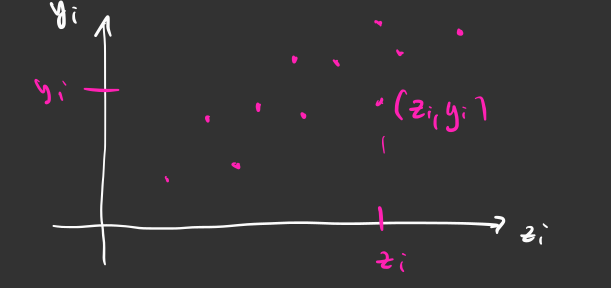
\includegraphics[width=0.5\linewidth]{curve-fitting}
	}
\end{frame}
\begin{frame}
	\Hide{	\textbf{Question:}
		Is there a ``significant'' relation between the $z_i$ and $y_i$?\\~\\
		Let us consider the $z_i$ as input (independent/explanatory/exogenous) variable,\\
		and the $y_i$ as output (dependent/predicted/response...) variable.\\~\\
		{Examples: $z_i$ = (temperature, light intensity), $y_i$ = plant height or $z_i$ = year, $y_i$ = global mean temperature}\\
		~\\~\\
		\textbf{Mathematically asking:} Is there a function $f$, so that
		$
		f(z_i)\cong y_i~\text{ for all $i=1,\ldots,m$?}
		$
		~\\~\\~\\
		\begin{minipage}[t]{0.48\textwidth}
			\underline{Exact fit:} \textbf{Interpolation}\\
			$$f(z_i)=y_i~\forall i=1,\dots,m$$
			~\\
			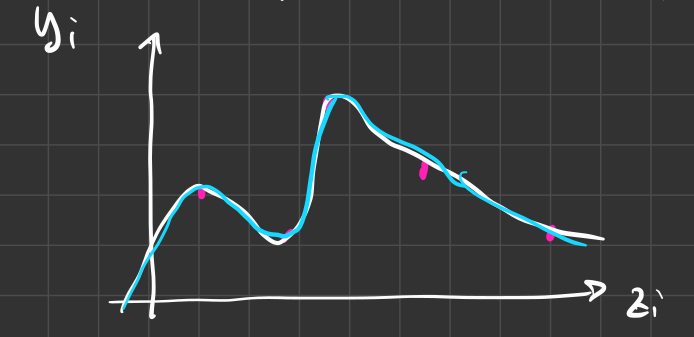
\includegraphics[width=0.7\linewidth]{interpolation-hand}
		\end{minipage}
		\begin{minipage}[t]{0.48\textwidth}
			\underline{Approximate fit:} \textbf{Regression/Smoothing}\\
			$$f(z_i)\approx y_i~\forall i=1,\dots,m$$
			~\\
			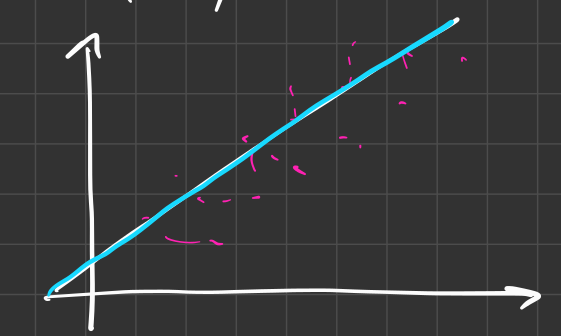
\includegraphics[width=0.7\linewidth]{regression-hand}
		\end{minipage}
	}
\end{frame}
\begin{frame}
	~\\
	\Hide{
		In order to find such a fit, we need to restrict ourselves to certain classes of functions $f$. With other words we need to assume a certain ''model'':\\
		$$z_i\stackrel{f}{\mapsto}y_i$$\\
		~\\
		In this course we will consider models of the following kind:
		$$
		f:\mathbb{R}\rightarrow\mathbb{R},~~f(z):=\sum_{k=1}^{n}x_kf_k(z)
		$$
		\begin{itemize}
			\item[$\rightarrow$] More precisely, we assume that the relation between the $z_i$ and the $y_i$ can be modeled by a \textit{linear combination}		 of $\underbrace{\text{some functions}~f_k:\mathbb{R}\rightarrow\mathbb{R}}_{\textit{\color{header}given by assumption}}$ 
			with 
			$\underbrace{\text{some coefficients/parameters}~x_k}_{\color{header}\textit{to be determined}~(f(z_i)\cong y_i)}$
			\item [] {\small (More generally $f,f_k\colon \R^k \to \R$. Important here is the fact that our model $f$ is linear combined from the $f_k$.)}
		\end{itemize}
		~\\
		\begin{example}[Polynomial Interpolation/Regression]
			One often considers a polynomial model:
			$$
			f_k(z) := z^{k-1},~~\text{so that}~~f(z)=x_1+x_2z+x_3z^2+\dots+x_nz^{n-1}
			$$
			For example, if $n=2$ then $f(z)=x_1+x_2z$ (an affine linear model).
		\end{example}
	}
\end{frame}

\begin{frame}
	~\\
	\Hide{
		\textbf{How does this translate into a linear system ``$Ax \cong b$''?}\\
		~\\
		For all measurements $(z_1,y_1),\dots,(z_m,y_m)$ we require:
		$$
		\sum_{k=1}^{n}x_kf_k(z_i)=f(z_i)\cong y_i~~\text{for all}~i=1,\dots,m
		$$
		Writing these equations row by row for each $i$-th measurement gives:
		\begin{align*}
		&\begin{matrix}
		i=1:&x_1f_1(z_1)+x_2f_2(z_2)+\dots+x_nf_n(z_1)&=y_1\\
		\vdots&\vdots&\vdots\\
		i=m:&x_1f_1(z_m)+x_2f_2(z_m)+\dots+x_nf_n(z_m)&=y_m
		\end{matrix}
		\end{align*}
		Using matrix notation, this system can be written as:
		$$
		\underbrace{
			\begin{pmatrix}
			f_1(z_1)&\cdots&f_n(z_1)\\
			\vdots&\ddots&\vdots\\
			f_1(z_m)&\cdots&f_n(z_m)
			\end{pmatrix}}_{=:A\in\mathbb{R}^{m\times n}}
		\underbrace{\begin{pmatrix}x_1\\x_2\\\vdots\\x_n\end{pmatrix}}_{=:x\in\mathbb{R}^n}
		\cong\underbrace{\begin{pmatrix}y_1\\\vdots\\y_m\end{pmatrix}}_{=:b\in\mathbb{R}^m} 
		~~~\Leftrightarrow~~~
		Ax\cong b
		$$
		~\\
		$\rightarrow$ Also revisit Example \ref{ex:interpolation}.
	}
\end{frame}

\begin{frame}
	~\\
	\Hide{
		\begin{minipage}[t]{0.48\textwidth}
			\underline{Exact:} \textbf{Interpolation}
			$$
			Ax=b
			$$
		\end{minipage}
		%%
		\begin{minipage}[t]{0.48\textwidth}
			\underline{Approximate:} \textbf{Regression}
			$$
			Ax\approx b
			$$
			A common approach to address a regression problem is a linear least squares formulation:
			\begin{align*}
			\min_{x\in\mathbb{R}^n}~\|Ax-b\|_2^2 ~&=~\sum_{i=1}^m(Ax-b)_i^2\\
			&=~\sum_{i=1}^m(f(z_i)-y_i)^2
			\end{align*}
			~\\
			\begin{figure}
				\centering
				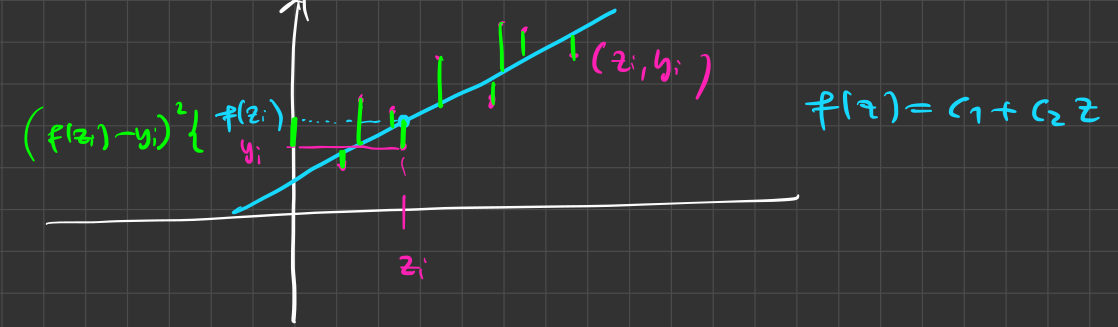
\includegraphics[width=1.1\linewidth]{regression-linear}
			\end{figure}
			
		\end{minipage}
		
		
	}
\end{frame}

\begin{frame}
	\Subsubsection{Existence and Uniqueness Analysis}
	\Hide{
		Let us consider the following cases:\\
		\begin{figure}
			\centering
			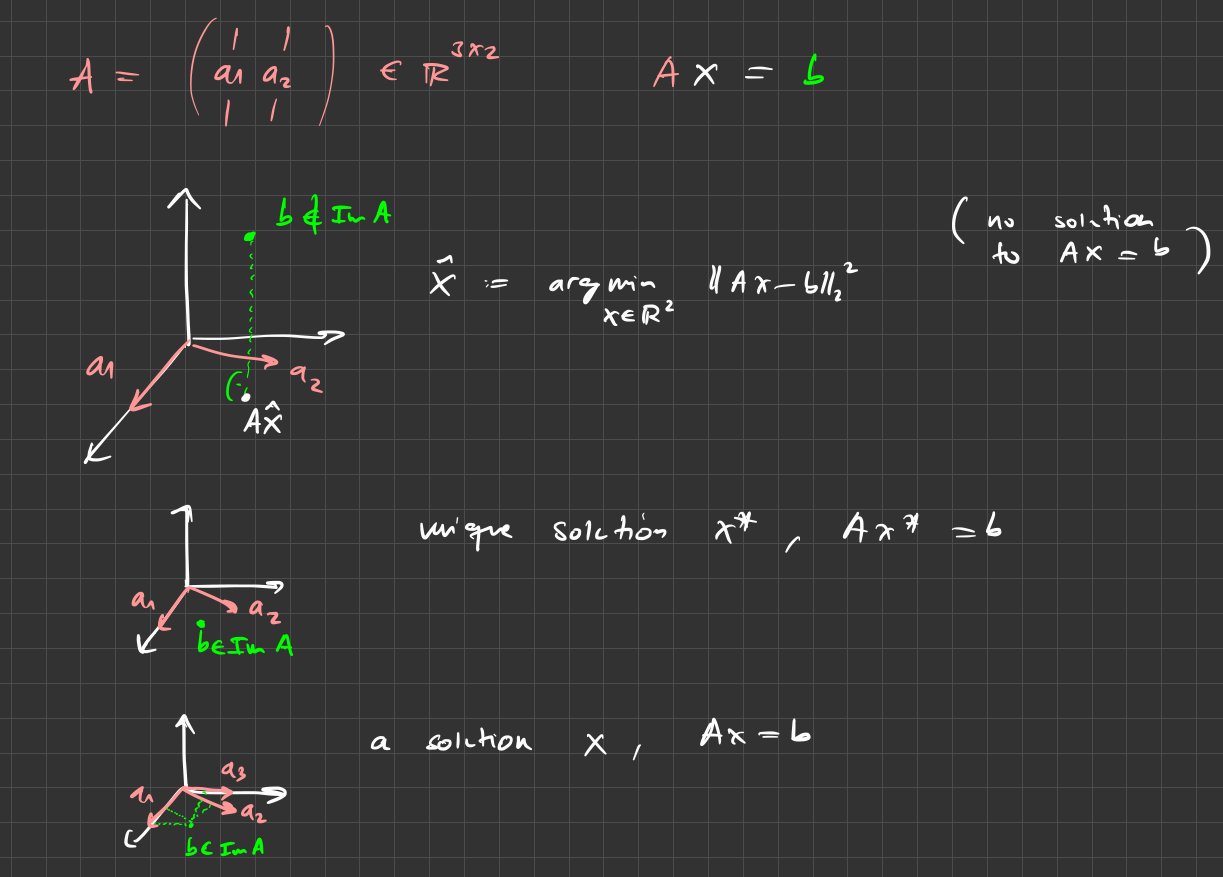
\includegraphics[width=0.85\linewidth]{existence-uniqueness-linsys}
			%	\caption{}
			%	\label{fig:existence-uniqueness-linsys}
		\end{figure}
		
		
		
	}
\end{frame}
\begin{frame}
	\textit{Summary}\\~\\
	\textbf{Aim:} \vspace*{-0.5cm}
	\begin{center}
		\textit{Given $A\in\mathbb{R}^{m\times n}$ ($m\neq n$ possible) and $b\in\mathbb{R}^m$,
			find $x\in\mathbb{R}^n$ such that\\
			$Ax=b.$}
	\end{center}
	\Hide{Here:
		\begin{itemize}
			\item[$m$]$=~\sharp$ equations $=~\sharp$ measurements $=$ length of the column vectors\\
			\item[$n$]$=~\sharp$ unknowns $=~\sharp$ parameters $=~\sharp$ columns\\
		\end{itemize}
		~~~~~~$\begin{matrix}~&{\color{cyan}n}\\A=~{\color{cyan}m}&\begin{pmatrix}|&~&|\\a_1&\cdots&a_n\\|&~&|\end{pmatrix}\end{matrix}$,~~~with image Im$(A)=\{Ax:\in\mathbb{R}^n\}~=$ span$(a_1,\dots,a_n)$\\
		~\\~\\
		Let us define the solution set
		$$S:=\{x\in\mathbb{R}^n:Ax=b\}~=~f_A^{-1}(\{b\}),$$
		then there are three possible states, namely,
		$$
		|S|=~\begin{cases}
		&0~:~\text{``no solution'', if~~}b\notin\text{Im}(A)\\
		&1~:~\text{``unique solution'', if~~}b\in\text{Im}(A)~\text{and independent columns}~(\text{ker}(A)=\{0\})\\
		&\infty~:~\text{``infinitely many solutions'', if~~}b\in\text{Im}(A)~\text{and dependent columns}~(\text{ker}(A)\neq\{0\})
		\end{cases}
		$$
		For a given $b$, observe the relations between image and existence as well as kernel and uniqueness. In fact,
		$b\in$ or $\notin\text{Im}(A)$ decides if solutions \textbf{exist} and \text{ker}(A) $=$ or $\neq~\{0\}$ gives the solutions' \textbf{uniqueness}.}
\end{frame}
%
%
\begin{frame}
	\Hide{
		Quick clarification:\\~\\
		Let $\ker(A)\neq \{0\}$, then there exists a $w \in \Rn$ so that $$A (\alpha w)= 0$$ for \textit{all} scalars $\alpha \in \R $.\\~\\
		If $b\in\im(A)$, then there exists an $x \in \Rn$, so that $$Ax = b.$$
		Adding these two equations gives
		$$A(x + \alpha w) = b ~~~\forall \alpha \in \R .$$ 
		With other words, we find infinitely many solutions.\\~\\
		Another equivalent argument in view of Lemma \ref{lem:linear-independence}: A nontrivial kernel implies that the columns are linearly dependent and thus vectors in their span are not uniquely combined. Now we see that this already implies infinitely many ways to linearly combine the columns of $A$ to obtain $b$ (assumed $b$ lies in there span).
	}
\end{frame}


\begin{frame}
	\Subsection{More on Image and Kernel}
Let us fix $\F = \R$ in this section. In this subsection we derive some more results on the kernel 
	$$\ker(A) = \{x\in \Rn: Ax = 0\} \subset \Rn$$ 
	and the image 
	$$\im(A) = \{Ax: x \in \Rn \} \subset \Rm.$$ 
 These results prove useful in later sections; in particular when we talk about the singular value decomposition.
	~\\~\\~\\
	\textbf{The Four Fundamental Subspaces}\\~\\
	In the context of a matrix $A \in \Rmn$ there are four subspaces that stand out:
	\begin{align*}
	  \ker(A)  ~~~\bot~~~&\im(A^\top)\\
	  \im(A) ~~~\bot~~~&\ker(A^\top).
	\end{align*}
	\Hide{The big picture of linear algebra:\\
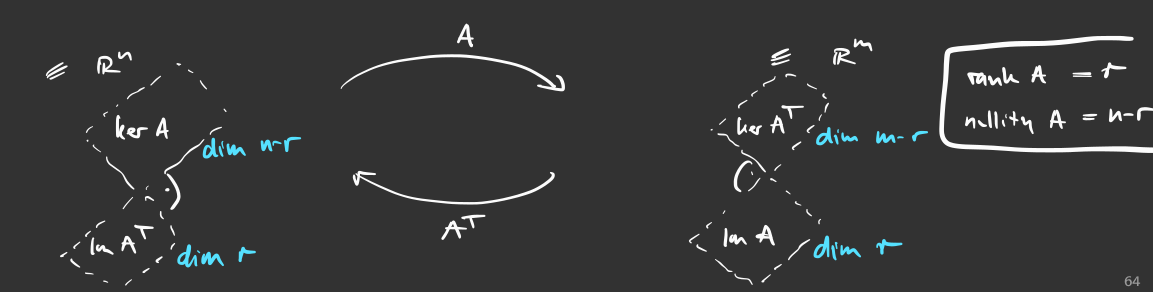
\includegraphics[width=0.9\linewidth]{media/bigpic-la}
}	
\end{frame}

\begin{frame}
\begin{example}\label{ex:bigPicture-LA}
		Let us consider
	$$A = \begin{pmatrix}1&2\\3&6\end{pmatrix}	,~~~~A^\top= \begin{pmatrix}1&3\\2&6\end{pmatrix}$$
	\Hide{
Then we find\\
\begin{minipage}[t]{0.48\textwidth} \small
\begin{align*}
\im(A) &= \text{span} \begin{pmatrix}1\\3\end{pmatrix}\\
\ker(A) &= \{x\in\R^2: Ax = 0\}\\
&= \{x\in\R^2:  x_1\begin{pmatrix}1\\3\end{pmatrix} +  x_2\begin{pmatrix}2\\6\end{pmatrix} = 0\} \\
&= \{x\in\R^2: 1x_1 + 2x_2 = 0\} \\
&= \{x\in\R^2: x_1 = - 2x_2\} \\
&= \spann \begin{pmatrix}-2\\1\end{pmatrix}
\end{align*}
\end{minipage}
\begin{minipage}[t]{0.48\textwidth} \small
\begin{align*}
\im(A^\top) &= \spann \begin{pmatrix}1\\2\end{pmatrix}\\
\ker(A^\top) &= \{x\in\R^2: Ax = 0\}\\
&= \{x\in\R^2: 1x_1 + 3x_2 = 0\}\\
&= \{x\in\R^2:  x_1 = - 3x_2 \}\\
&= \spann \begin{pmatrix}-3\\1\end{pmatrix}
\end{align*}
\end{minipage}
~\\
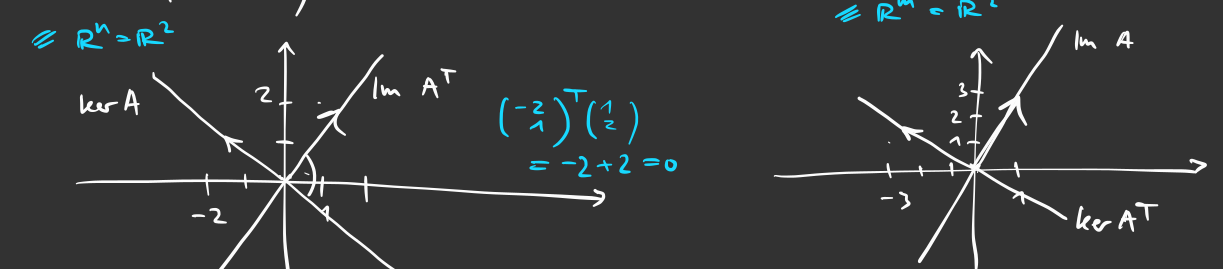
\includegraphics[width=0.9\linewidth]{media/ex-bigPicture-LA}
}
\end{example}

\end{frame}

\begin{frame}
	We need another definition:
	\begin{defi}[Orthogonal subspaces]
		 Let $U,V \subset \R^n$ be two subspaces.  
		 \begin{itemize}
		 	\item[i)] We call $U$ and $V$ \textbf{orthogonal} ($U \bot V$) if $u^\top v = 0$ for all $u \in U, v\in V$.
		 	\item[ii)] We call 
		 	$$U^\bot := \{x\in  \R^n \colon x^\top u = 0 ~~\forall ~u \in U\} $$
		 	the \textbf{orthogonal complement} of $V$ in $\Rn$.
		 \end{itemize}
	\end{defi}
~\\
 \textit{Exercise:} {\color{satzrot}Show that $(U^\bot)^\bot = U$ and $U \bot U^\bot$.}
\begin{example}\label{ex:orthogonalSubspaces}
	\Hide{~\\
i) $n=2$, $U := \text{span}({\begin{pmatrix}1\\0\end{pmatrix}}), V := \text{span}({\begin{pmatrix}0\\1\end{pmatrix}})$. Then
$$\forall u = \begin{pmatrix}u_1\\0\end{pmatrix} \in U, v= \begin{pmatrix}0\\v_2\end{pmatrix}\in V: u^\top v = u_1 \cdot 0 + 0 \cdot v_2 = 0. $$
Thus, $U \bot V$.
~\\
ii) $n=3$, $U := \text{span}(\begin{pmatrix}1\\0\\0\end{pmatrix}, \begin{pmatrix}0\\1\\0\end{pmatrix})$.
%Then  $U= \im(A)$ with $A = \begin{pmatrix}1&0\\0&1\\0&0\end{pmatrix} $. 
Thus for any $u\in U$ we have $u =  \begin{pmatrix}u_1\\u_2\\0\end{pmatrix}$. Then
\begin{align*}
U^\bot &= \{x\in  \R^3 \colon x^\top u = 0 ~~\forall ~u \in U\} 
 =  \{x\in  \R^3 \colon x_1u_1 + x_2u_2 = 0 ~~\forall ~u_1, u_2 \in \R \} \\
 &=  \{x\in  \R^3 \colon x_1=x_2=0 \} ~~~~\text{\color{cyan}\it(choose $u_1=1, u_2=0$ and $u_1=0, u_2=1$)}\\
 &= \text{span}(\begin{pmatrix}0\\0\\1\end{pmatrix}).
\end{align*}
\demo{draw pictures}
}
\end{example}

\end{frame}

\begin{frame}
	We now prove the orthogonality relation between the four fundamental subspaces:
\begin{lemma}\label{lem:ortho-fundamental-subspaces}
	Let $A \in \Rmn$. Then
		\begin{align*}
	\im(A)^\bot =\ker(A^\top)~~~\text{and}~~~\ker(A)^\bot=\im(A^\top)	.
	\end{align*}
	In words, $\ker(A^T)$ is the \textbf{orthogonal complement} of $\im(A)$ in $\Rm$ and $\im(A^T)$ is the orthogonal complement of $\ker(A)$ in $\Rn$.
\end{lemma}
\Hide{ 
\begin{proof}
We show the first equation. The orthogonal complement of $\im(A)$ can be characterized as
\begin{align*}
\im(A)^\bot = \{y\in\Rm: z^\top y = 0 ~~\forall z \in \im(A)\} = \{y\in\Rm: x^\top A^\top y = 0 ~~\forall x \in \Rn\}.~~~~\text{\small\it \color{cyan}(simply write $z = Ax$)}
\end{align*}	
Now we show mutual subset relation. First,
\begin{align*}
y \in \im(A)^\bot &\Rightarrow \forall x\in \Rn: x^\top(A^\top y) = 0\\
&\Rightarrow \text{for the basis vectors~} e_1,\ldots, e_n:    e_i^\top(A^\top y) = (A^\top y)_i = 0\\
&\Rightarrow   A^\top y = 0~\text{,i.e.,}~~y\in\ker(A^\top).
\end{align*}
Second, 
\begin{align*}
y \in \ker(A^\top) &\Rightarrow  A^\top y = 0\\
&\Rightarrow \forall x\in \Rn: x^\top(A^\top y) = (Ax)^\top y= 0\\
&\Rightarrow y \in \im(A)^\bot.
\end{align*}
The second equation follows from applying the first equation to  $C = A^T$ and $(U^\bot)^\bot = U$.
\end{proof}
}
% 
%We have that $\ker(A^T)$ is the \textbf{orthogonal complement} of $\im(A)$ in $\Rm$ and we write
%$$ \im(A)=\ker(A^T)^\bot ~~~\text{or}~~~\im(A)^\bot = \ker(A^T).$$
%Analogously $\ker(A)$ is the orthogonal complement of $\im(A^T)$ in $\Rn$ and we write
%$$\ker(A) = \im(A^T)^\bot~~~\text{or}~~~\ker(A)^\bot = \im(A^T).$$ 
\end{frame}

\begin{frame}
	In terms of the transpose matrix we find two more characterizations of the image and kernel:
	\begin{lemma}\label{lem:kernel-image}
			Let $A \in \Rmn$. Then
		\begin{align*}
		i)~~~\ker(A) &= \ker(A^\top A)~~~(\text{and}~~~\ker(A^\top) = \ker(AA^\top )),\\
		ii)~~~\im(A) & = \im(A A^\top)~~~(\text{and}~~~\im(A^\top) = \im(A^\top A)).
 		\end{align*}
	\end{lemma}
\Hide{
\begin{proof}
We only prove i) here. We show this by mutual subset relation:
\begin{itemize}
	\item \underline{``$\ker(A)\subseteq \ker(A^TA)$'':}\\
Let $x\in \ker(A) \stackrel{\textcolor{cyan}{\text{Def.}\ \ker(A)}}{\Rightarrow}Ax=0\Rightarrow A^TAx=0\stackrel{\textcolor{cyan}{\text{Def.}\ \ker(A^TA)}}{\Rightarrow}x\in \ker(A^TA)$.\\~\\
\item \underline{``$\ker(A^TA)\subseteq \ker(A)$'':}\\
Let $x\in \ker(A^TA) \stackrel{\textcolor{cyan}{\text{Def.}}}{\Rightarrow}A^TAx=0\Rightarrow \underbrace{x^TA^TAx}_{\textcolor{cyan}{=\|{Ax}\|_2^2}}=0 \stackrel{\textcolor{cyan}{\text{norm}~ \|{\cdot}\|_2~ \text{is definite}}}{\Rightarrow}Ax=0 \stackrel{\textcolor{cyan}{\text{Def.}}}{\Rightarrow}x\in \ker(A)$.
\end{itemize}
Exercise: To prove ii) one can exploit the orthogonality of the subspaces as derived above.\\ 
The results for the transpose follow by applying the results to $C:=A^T$.
\end{proof}
}
{
~\\
\small 
\textbf{Remark}\\
The so-called Gram matrix $A^\top A$ plays a crucial role in many applications and also analysis, for instance
\begin{itemize}
	\item it plays a key role to derive the singular value decomposition
	\item it is the system matrix in the normal equation $A^\top A x=A^\top x $ for solving least squares problems
	\item in graph theory it appears as graph Laplacian
	\item if $A \approx \nabla$ (gradient), then $A^\top\approx \text{div}$ (divergence) and $A^\top A \approx \Delta$ (Laplacian)
\end{itemize}
}
\end{frame}

\begin{frame}
	A generalization of this result is given by the following lemma.
		\begin{lemma} \label{lem:kerImProducts}
		Let $A \in \Rmn$. Then
\begin{itemize}
	\item[i)] For a matrix $B \in \R^{\ell\times m}$ with $\ker(B) = \{0\}$ 
	%$m \leq \ell$ and $\rank(B)=m$ 
	(``injective'') we have
				$$\ker(BA) = \ker(A). $$
	\item[ii)] For a matrix $C \in \R^{n\times k}$ with $\im(C)=\R^n$
	% $n \leq k$ and $\rank(C)=n$ 
	(``surjective'') we have
$$\im(AC) = \im(A). $$
\end{itemize}
	\end{lemma}

	\Hide{\small
		\begin{center}
		~\\	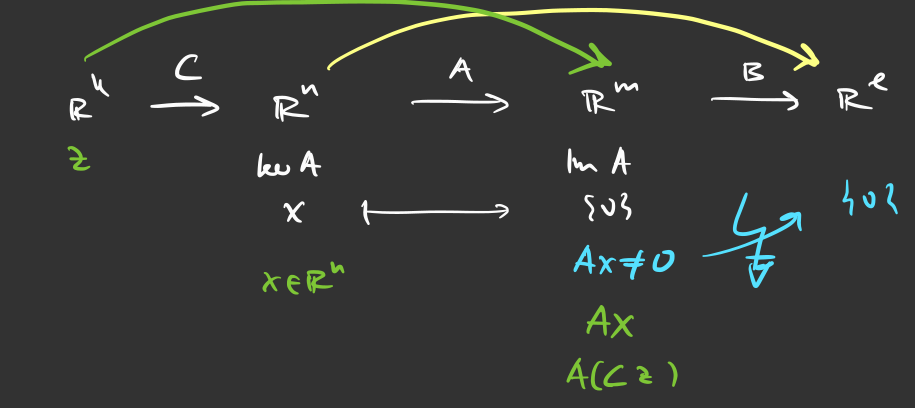
\includegraphics[width=0.4\linewidth]{media/la-concatenate-mats}\\
		\end{center}
	\begin{proof}	
We show mutual subset relation:\\
i)
\underline{``$\ker(BA)\subseteq \ker(A)$'':}\\
 	Let $BA x = B(A x) =0$. Since by assumption $\ker(B) = \{0\}$, we have $Ax = 0$.\\
	\underline{``$\ker(A)\subseteq \ker(BA)$'':}\\
	For $Ax = 0$ we also have $BAx = B(Ax)= B 0 = 0$.\\
ii)	
\underline{``$\im(AC)\subseteq \im(A)$'':}\\
Let $y = ACx = A (Cx)$ for some $x\in \R^k$. Then with $z := Cx \in \Rn$ we see that $y = Az$ is in the image of $A$.   \\
\underline{``$\im(A)\subseteq \im(AC)$'':}\\
Let $y = Az$ for some $z\in\Rn$. Since $\im(C)=\R^n$
%$\rank(C)=n$, so that its columns form a basis for $\Rn$, 
we find some coefficients $x\in\R^k$ so that $z=Cx$. With $y = ACx$ we see that $y$ is in the image of $AC$.
\end{proof}
}
\end{frame}

\begin{frame}
\textbf{Example}
~\\~\\
%\Hide{	
	The typical context to apply Lemma \ref{lem:kerImProducts} occurs when we have a decomposition of a matrix $A$ and want to investigate its kernel and its image.
	~\\~\\
	 For example, consider the reduced QR decomposition $A = QR$, where $Q \in \Rmn$ contains orthonormal columns and $R \in \Rnn$ is upper triangular. Suppose that $A$ has full rank, i.e., $\rank(A)= n$, so that $R$ is invertible (in particular $\rank(R)=n$ and $\ker(R)=\{0\}$). We thus find by Lemma \ref{lem:kerImProducts} i) that
	$$\ker(A) = \ker(QR) = \ker(R) = \{0\} $$
	and by Lemma \ref{lem:kerImProducts} ii) that
	$$\im(A) = \im(QR)= \im(Q).$$
	With other words, the $n$ columns in $Q$ are an orthonormal basis for the image $\im(A)$ of $A$.
%}
\end{frame}



